 \chapter{Sensitivity to Atmospheric Neutrinos Oscillations} \label{chap:oscillation_parameter_measurement}

This chapter shows the impact that the improved PID has on a measurement of atmospheric neutrino oscillations.
The newly developed PID variable \textit{GBM probability} based on the multivariate classification method explained in Chapter~\ref{chap:improving_pid} is compared to the univariate PID discriminator \textit{$\chi^2$-ratio} that was used in the past to show the improvement.
Section~\ref{sec:analysis_principle} describes the binned likelihood analysis strategy and how the parameter uncertainties are estimated.
Section~\ref{sec:pid_optimization} illustrates the binning optimization procedure.
In Section~\ref{sec:sensitivity_improvement}, the sensitivities to the atmospheric mixing parameters $\Delta \rm{m}^{2}_{32}$ and $\theta_{23}$ are presented.


\section{Analysis Strategy} \label{sec:analysis_principle}

The extraction of neutrino oscillation parameters is based on the dependence of the oscillation probability on the neutrino energy and the traveled distance of the neutrino, as explained in Section~\ref{sec:neutrino_oscillations}.
The traveled distance of a neutrino that is detected in IceCube is related to its incoming zenith angle and therefore we can illustrate the oscillation probability as a function of energy $E$ and cosine of the zenith angle $\theta_z$, $\mathrm{cos}\,\theta_z$.
Figure~\ref{fig:muon_surv_prob} shows the muon neutrino survival probability for a chosen set of oscillation parameters.
A zenith angle of $\theta_z=\pi$ ($\mathrm{cos}\,\theta_z=-1$) corresponds to a neutrino coming from the negative z direction.
The green bands are the oscillation pattern that we want to observe. Due to the minimum neutrino detection energy threshold of approximately 5\,GeV in DeepCore, the signal we can detect is in the energy region of 20-40\,GeV for up-going neutrinos.

\begin{figure}[h]
    \centering
    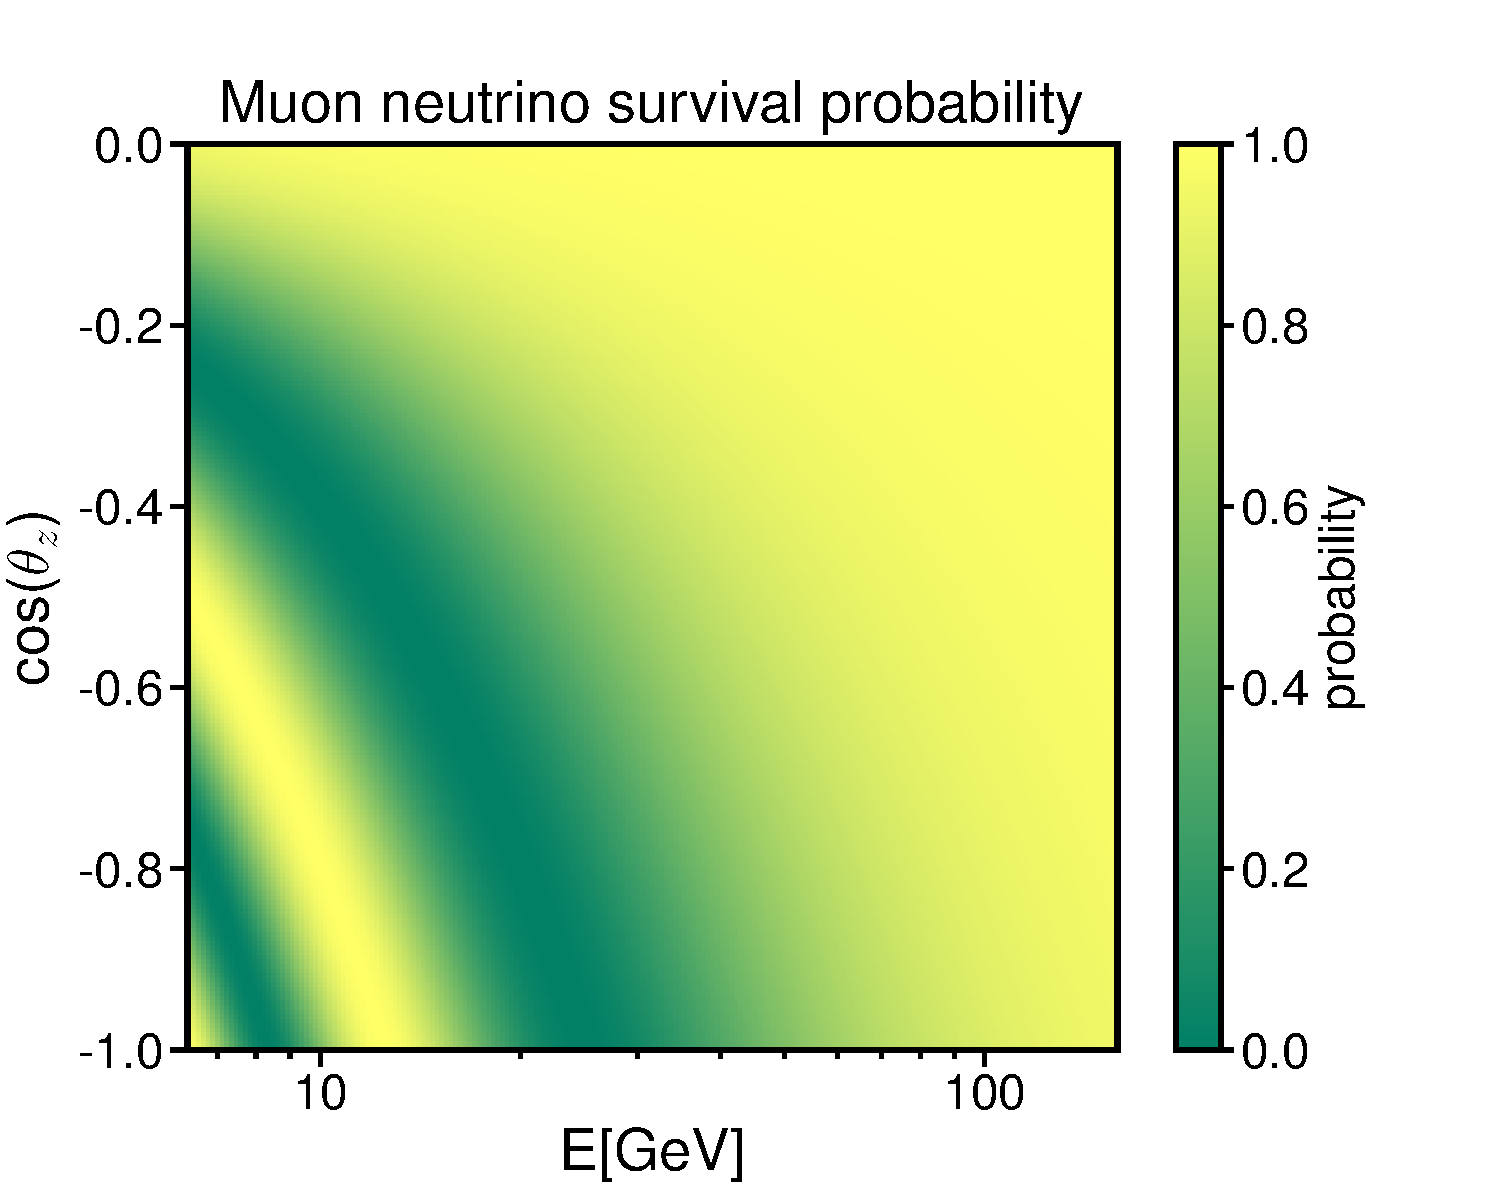
\includegraphics[trim = 00 00 00 00, clip, width=0.75\linewidth]{figures/oscillaogram_muon.pdf}
    \caption[Muon neutrino survival probability in two-flavor approximation]{Muon neutrino survival probability in two-flavor approximation as in Equation~\ref{eq:survival_probability} with $\Delta\mathrm{m}^2_{32}=2.42\cdot10^{-3}$\,eV$^2$ and sin$^2\theta_{23}=0.538$.}
    \label{fig:muon_surv_prob}
\end{figure}

\subsection{Binned Poisson Likelihood} \label{sec:likelihood_estimation}

A binned likelihood method is used to determine the neutrino oscillation parameters.
For this method, the observed events are binned in three-dimensional histograms by $E$, $\mathrm{cos}\,\theta_z$ and PID.
Assuming a Poisson distribution of event counts in each bin we can fit the oscillation parameters by minimizing the logarithmic likelihood
\begin{equation}
    -\log(\mathcal{L}) = \sum^N_{i=1}\mu_i(\theta, \phi)-n_i\log(\mu_i(\theta, \phi)) + \sum_k \frac{(\phi_k-\phi^0_k)^2}{2\sigma_{\phi_k}^2},
    \label{eq:maximum_llh_method}
\end{equation}
where $n_i$ is the number of observed data events and $\mu_i(\theta, \phi)$ is the expected number of events in the $i^{th}$ bin depending on the physics parameters of interest $\theta$ and the nuisance parameters $\phi$.
The second term in Equation~\ref{eq:maximum_llh_method} accounts for prior knowledge on the nuisance parameters.
It is the sum of Gaussian penalties, where $\phi^0_k$ is the central value of the $k^{th}$ nuisance parameter and $\sigma_{\phi_k}$ its Gaussian standard deviation.
The priors are taken from model predictions or from independent measurements.
As minimizer we use the Sequential Least SQuares Programming (SLSQP) method provided by the SciPy library \cite{2019arXiv190710121V}.

The expected number of events of the bin content is calculated from simulated events using forward folding \cite{ATerliuk}.
Forward folding means that the weight of each simulated event is modified to match the expected distribution under assumption of a set of parameters.
The expected oscillated flux of a given neutrino flavor $\nu_\alpha$ is calculated from the $k^{th}$ simulated event as the composition of the atmospheric fluxes multiplied by the probabilities to oscillate into the neutrino flavor of interest.
The flux is given by
\begin{equation}
    \Phi_{\nu_\alpha}^{k,{\mathrm{osc}}} = \Phi_{\nu_e}^{k}\cdot P^\mathrm{osc}_{\nu_e\rightarrow\nu_\alpha} + \Phi_{\nu_\mu}^{k}\cdot P^\mathrm{osc}_{\nu_\mu\rightarrow\nu_\alpha},
    \label{eq:neutrino_flux}
\end{equation}
where $\Phi_{\nu_e}^{k}$ and $\Phi_{\nu_\mu}^{k}$ are the atmospheric fluxes corresponding to the $k^{th}$ event and $P^\mathrm{osc}_{\nu_e\rightarrow\nu_\alpha}$ and $P^\mathrm{osc}_{\nu_\mu\rightarrow\nu_\alpha}$ are the oscillation probabilities to the flavor $\nu_\alpha$.
The probabilities are modified by the neutrino mixing parameters, while the atmospheric fluxes depend on the flux model and its governing parameters \cite{PhysRevD.92.023004_Honda_Flux}.
Multiplying the flux for a given neutrino flavor by the weight factor that incorporates interaction effects (detector response, cross-section etc.) yields the total weight for each event $k$ and flavor $\alpha$
\begin{equation}
    \omega^{k,\alpha} = \omega_0^{k,\alpha} \cdot \Phi_{\nu_\alpha}^{k,{\mathrm{osc}}},
    \label{eq:total_weight}
\end{equation}
where $\omega_0^{k,\alpha}$ is the weight factor. This is the weight factor that was already mentioned in Section~\ref{sec:gradient_boosting_classifier} used to re-weight the events to get a realistic distribution.
The total weight $\omega^{k,\alpha}$ has units of events per second. Binning all simulated events, taking into account their total weight, and multiplying the summed weight by the detector livetime, yields the expected number of events $\mu_i(\theta)$.


\subsection{Sensitivity Estimation} \label{sec:uncertainty_estimation}

To estimate the uncertainty on the physics parameters, we use an Asimov dataset \cite{2011EPJC...71.1554C}.
This means that the expected number of events and the number of observed data events in Equation~\ref{eq:maximum_llh_method} are both produced from the same simulation dataset.
We choose a set of physics parameters $\hat{\theta}$ for the production of the data events.
As a result, these injected parameters $\hat{\theta}$ should be perfectly recovered when performing the maximum likelihood fit. 
The shape of the uncertainty region is estimated by profiling the likelihood with respect to the physics parameters of interest $\theta$.
For any set of $\theta$ the likelihood value is calculated using Equation~\ref{eq:maximum_llh_method}.
With this likelihood we can construct the \textit{test statistic} (TS) used in this work, which is defined as
\begin{equation}
    -2\Delta \log\mathcal{L}(\theta) = -2\Big( \log\mathcal{L}(\theta) - \log\mathcal{L}(\hat\theta) \Big),
\end{equation}
where $\hat\theta$ are the injected parameters and $\theta$ are the set of parameters to be probed.
Furthermore, we apply Wilk's theorem \cite{wilks1938} by assuming that the TS is approximated by a $\chi^2$-distribution.
For a $\chi^2$-distribution with two degrees of freedom the $68$\,\% and $90$\,\% confidence levels (C.L.) are found at values 2.28 and 4.61, respectively. 
Parameters with a TS exceeding these values can be rejected with the given C.L..


\subsection{Systematic Uncertainties} \label{sec:systematics}

The impact of systematic uncertainties is incorporated in the analysis by treating them as nuisance parameters implemented in Equation~\ref{eq:maximum_llh_method}.
They have an effect on the shape and normalization of the expected event distributions.
The systematic uncertainties can be roughly categorized in the following groups depending on their origin:
The initial, un-oscillated flux of atmospheric neutrinos, the neutrino-nucleon interaction cross-section, the neutrino flavor oscillation parameters and the detector response.
The discussion of the impact of the systematic uncertainties follows closely the description in \cite{2019PhRvD..99c2007A}.


\paragraph{Atmospheric neutrino flux:}

A detailed study of the uncertainties resulting from the calculation of the neutrino flux has been performed in \cite{2006PhRvD..74i4009B}.
Depending on their origin, they can depend on $E$, $\cos\theta_z$ and particle species.
The uncertainties on the neutrino energy spectra resulting from uncertainties in modelling the cosmic ray energy spectra are purely $E$ dependent.
Uncertainties in the $\pi$- and $k$-meson production lead to uncertainties that are $E$, $\cos\theta_z$ and particle species dependent.
The explicit parametrization of the atmospheric neutrino flux uncertainties is not discussed here but can be found in \cite{2019PhRvD..99c2007A}.
Additionally, there are uncertainties that are independent of $E$ and $\cos\theta_z$ that effect the total scaling of the neutrino flux.
Since these uncertainties are very large, they are not constrained but instead the total normalization of the neutrino flux is left as a free fit parameter.


\paragraph{Neutrino-nucleon interactions:}

From all the cross-section systematics that were tested, only two were not already degenerate with other systematic uncertainties.
The two are the axial mass form factors for CC quasi-elastic and resonant scattering.
They parameterize the quasi-elastic and resonant scattering cross-sections as described in \cite{Formaggio_Cross_Sections}.
Both of them are included as systematic uncertainties based on corrections calculated using GENIE \cite{2015arXiv151005494A}, which is the tool used to produce the neutrino interaction simulation.
Possible uncertainties in the hadronization processes of NC interactions are taken into account by adding a normalization factor for NC interactions.


\paragraph{Oscillation parameters:}

The oscillation model in this work uses the full, three-flavor formalism including three mixing angles, two mass-squared splittings and a CP violating phase (compare Equation~\ref{eq:PMNS_matrix}).
Since we are not sensitive to $\Delta \rm{m}^{2}_{21}$ and $\theta_{12}$ nor the CP violating phase $\delta_{CP}$, they are fixed.
The angle $\theta_{13}$ is treated as a systematic uncertainty. 
The atmospheric mixing parameters $\Delta \rm{m}^{2}_{32}$ and $\theta_{23}$ are free to fit.
The neutrino mass ordering is not known and for this work only normal mass ordering is considered.


\paragraph{}

Additionally, there are uncertainties related to the detector response and the atmospheric muon flux.
However, these systematics are not taken into account in this work.
Two sensitivity studies for atmospheric neutrino mixing are performed in this work: one without taking into account any systematic uncertainties and one taking into account the systematic uncertainties previously discussed.


\section{Analysis Binning} \label{sec:pid_optimization}

In this work we use the same $E$ and $\cos\,\theta_z$ binning as in previous analyses \cite{ATerliuk}.
The binning is the following: 11 logarithmically spaced bins in the $E$ range of $[10^{0.8},10^{2.2}]$\,GeV ($[6.31,158.49]$\,GeV) and 10 linearly spaced bins in the $\cos\,\theta_z$ range of $[-1.,0.]$.
The binning in the GBM probability must be optimized.
This is done by performing a scan over varying GBM probability cut values and choosing the value which yields the best result in terms of sensitivities.
The sensitivity studies are executed in the full three flavor model assuming vacuum oscillation.
The oscillation parameters injected are taken from NuFit 2.0 \cite{Gonzalez-Garcia2014} with maximum mixing $\theta_{23}=45\degree$ and 8.0\,years of livetime assuming normal mass ordering (i.e $m_3 > m_2 > m_1$).
The optimization is performed for the GBM probability as well as for the $\chi^2$-ratio.
Figure~\ref{fig:optimizing_two_bins} shows the results of the optimization processes.

\begin{figure}[h]
    \centering
    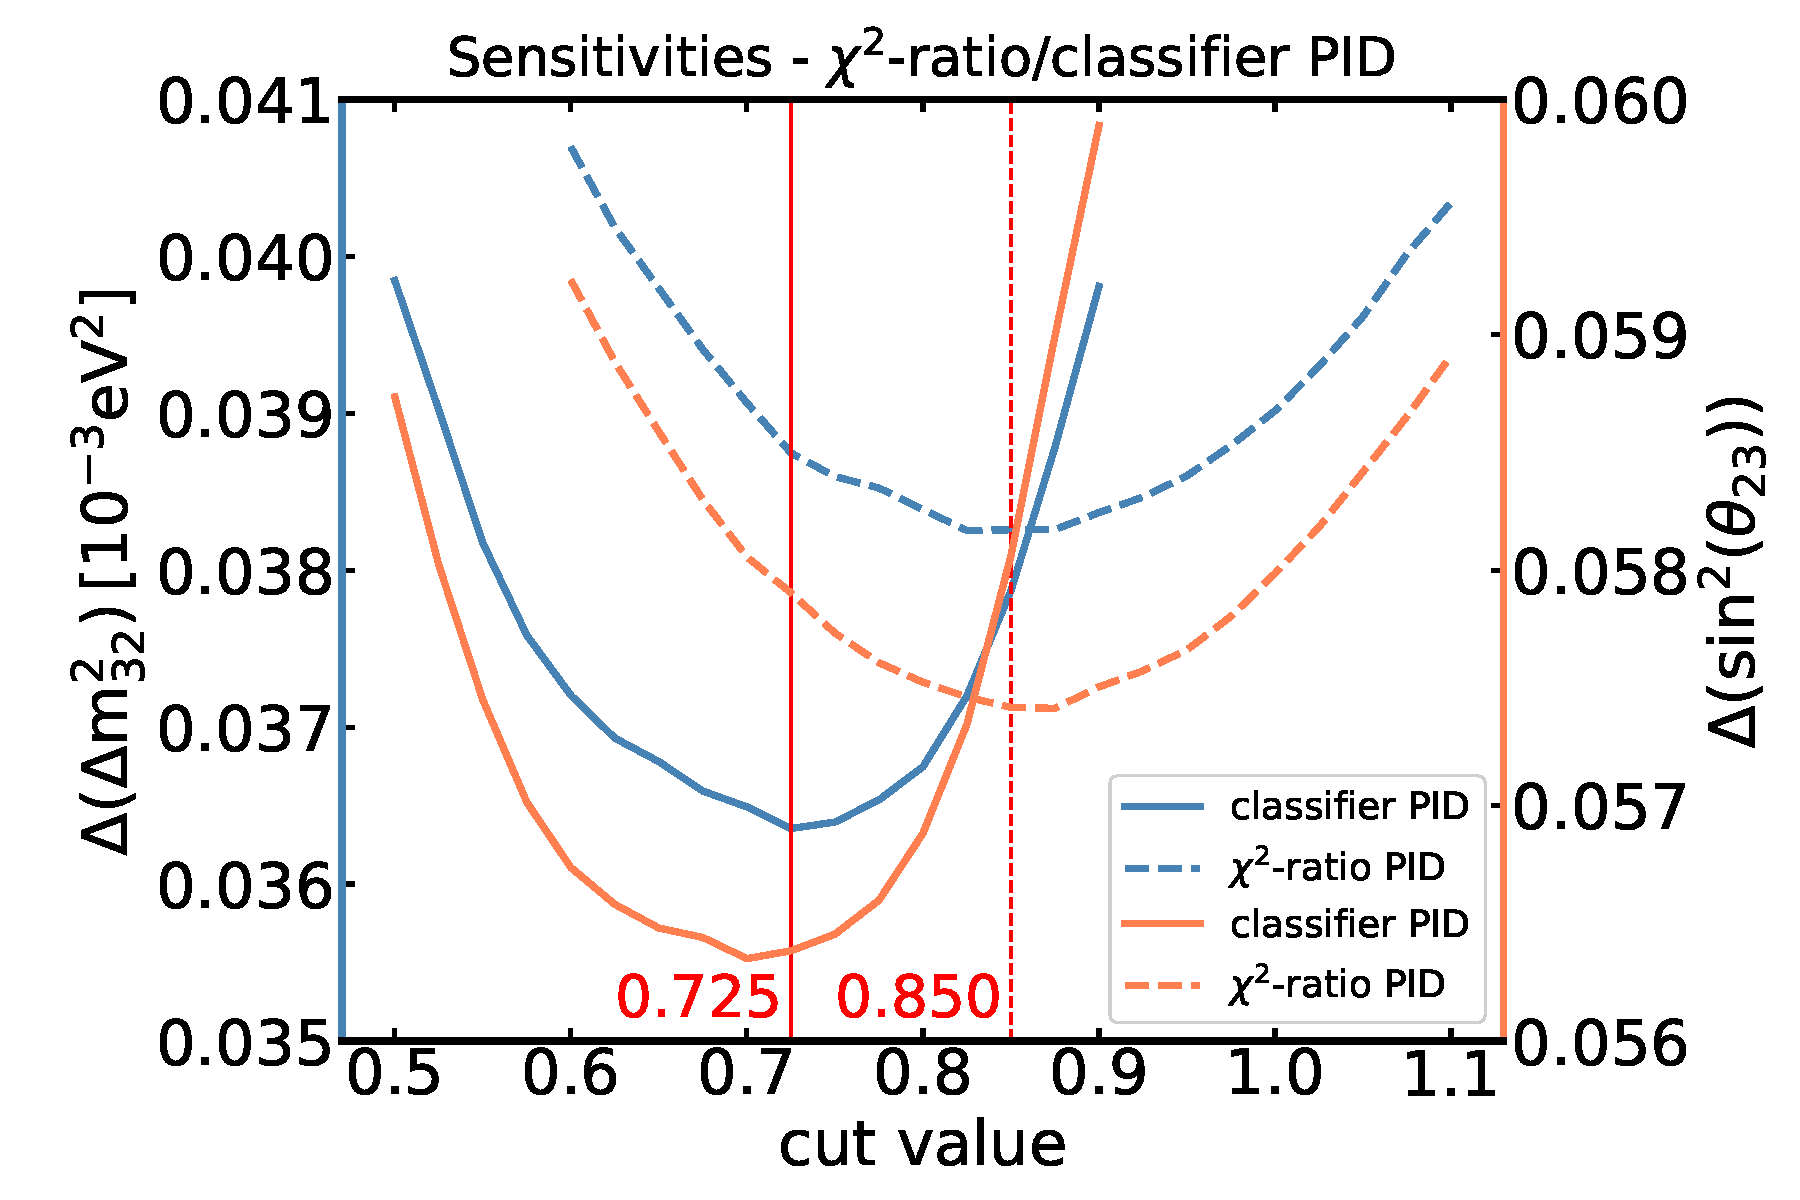
\includegraphics[width=0.8\linewidth]{figures/pid_optimization_combined.pdf}
    \caption[Sensitivity results of the two-bin PID cut optimization]
    {Sensitivity results of the two-bin PID cut optimization for the GBM probability (solid line) and the $\chi^2$-ratio (dashed line) with optimal cut value indicated in red. $\Delta(\Delta \mathrm{m}^{2}_{32})$ (blue) and $\Delta(\sin^{2}(\theta_{23}))$ (orange) are the sizes of the $68$\,\% C.L. for mixing angle and mass splitting, respectively.}
    \label{fig:optimizing_two_bins}
\end{figure}

For a binary binning, the optimal GBM probability cut is 0.725 and the optimal $\chi^2$-ratio cut is 0.85.
As can be observed, the new PID achieves better sensitivities at the chosen cut value.
In the following, these values will be used to split the sample in track bin and cascade bin to perform an oscillation measurement.

\begin{figure}[h!]
    \centering
    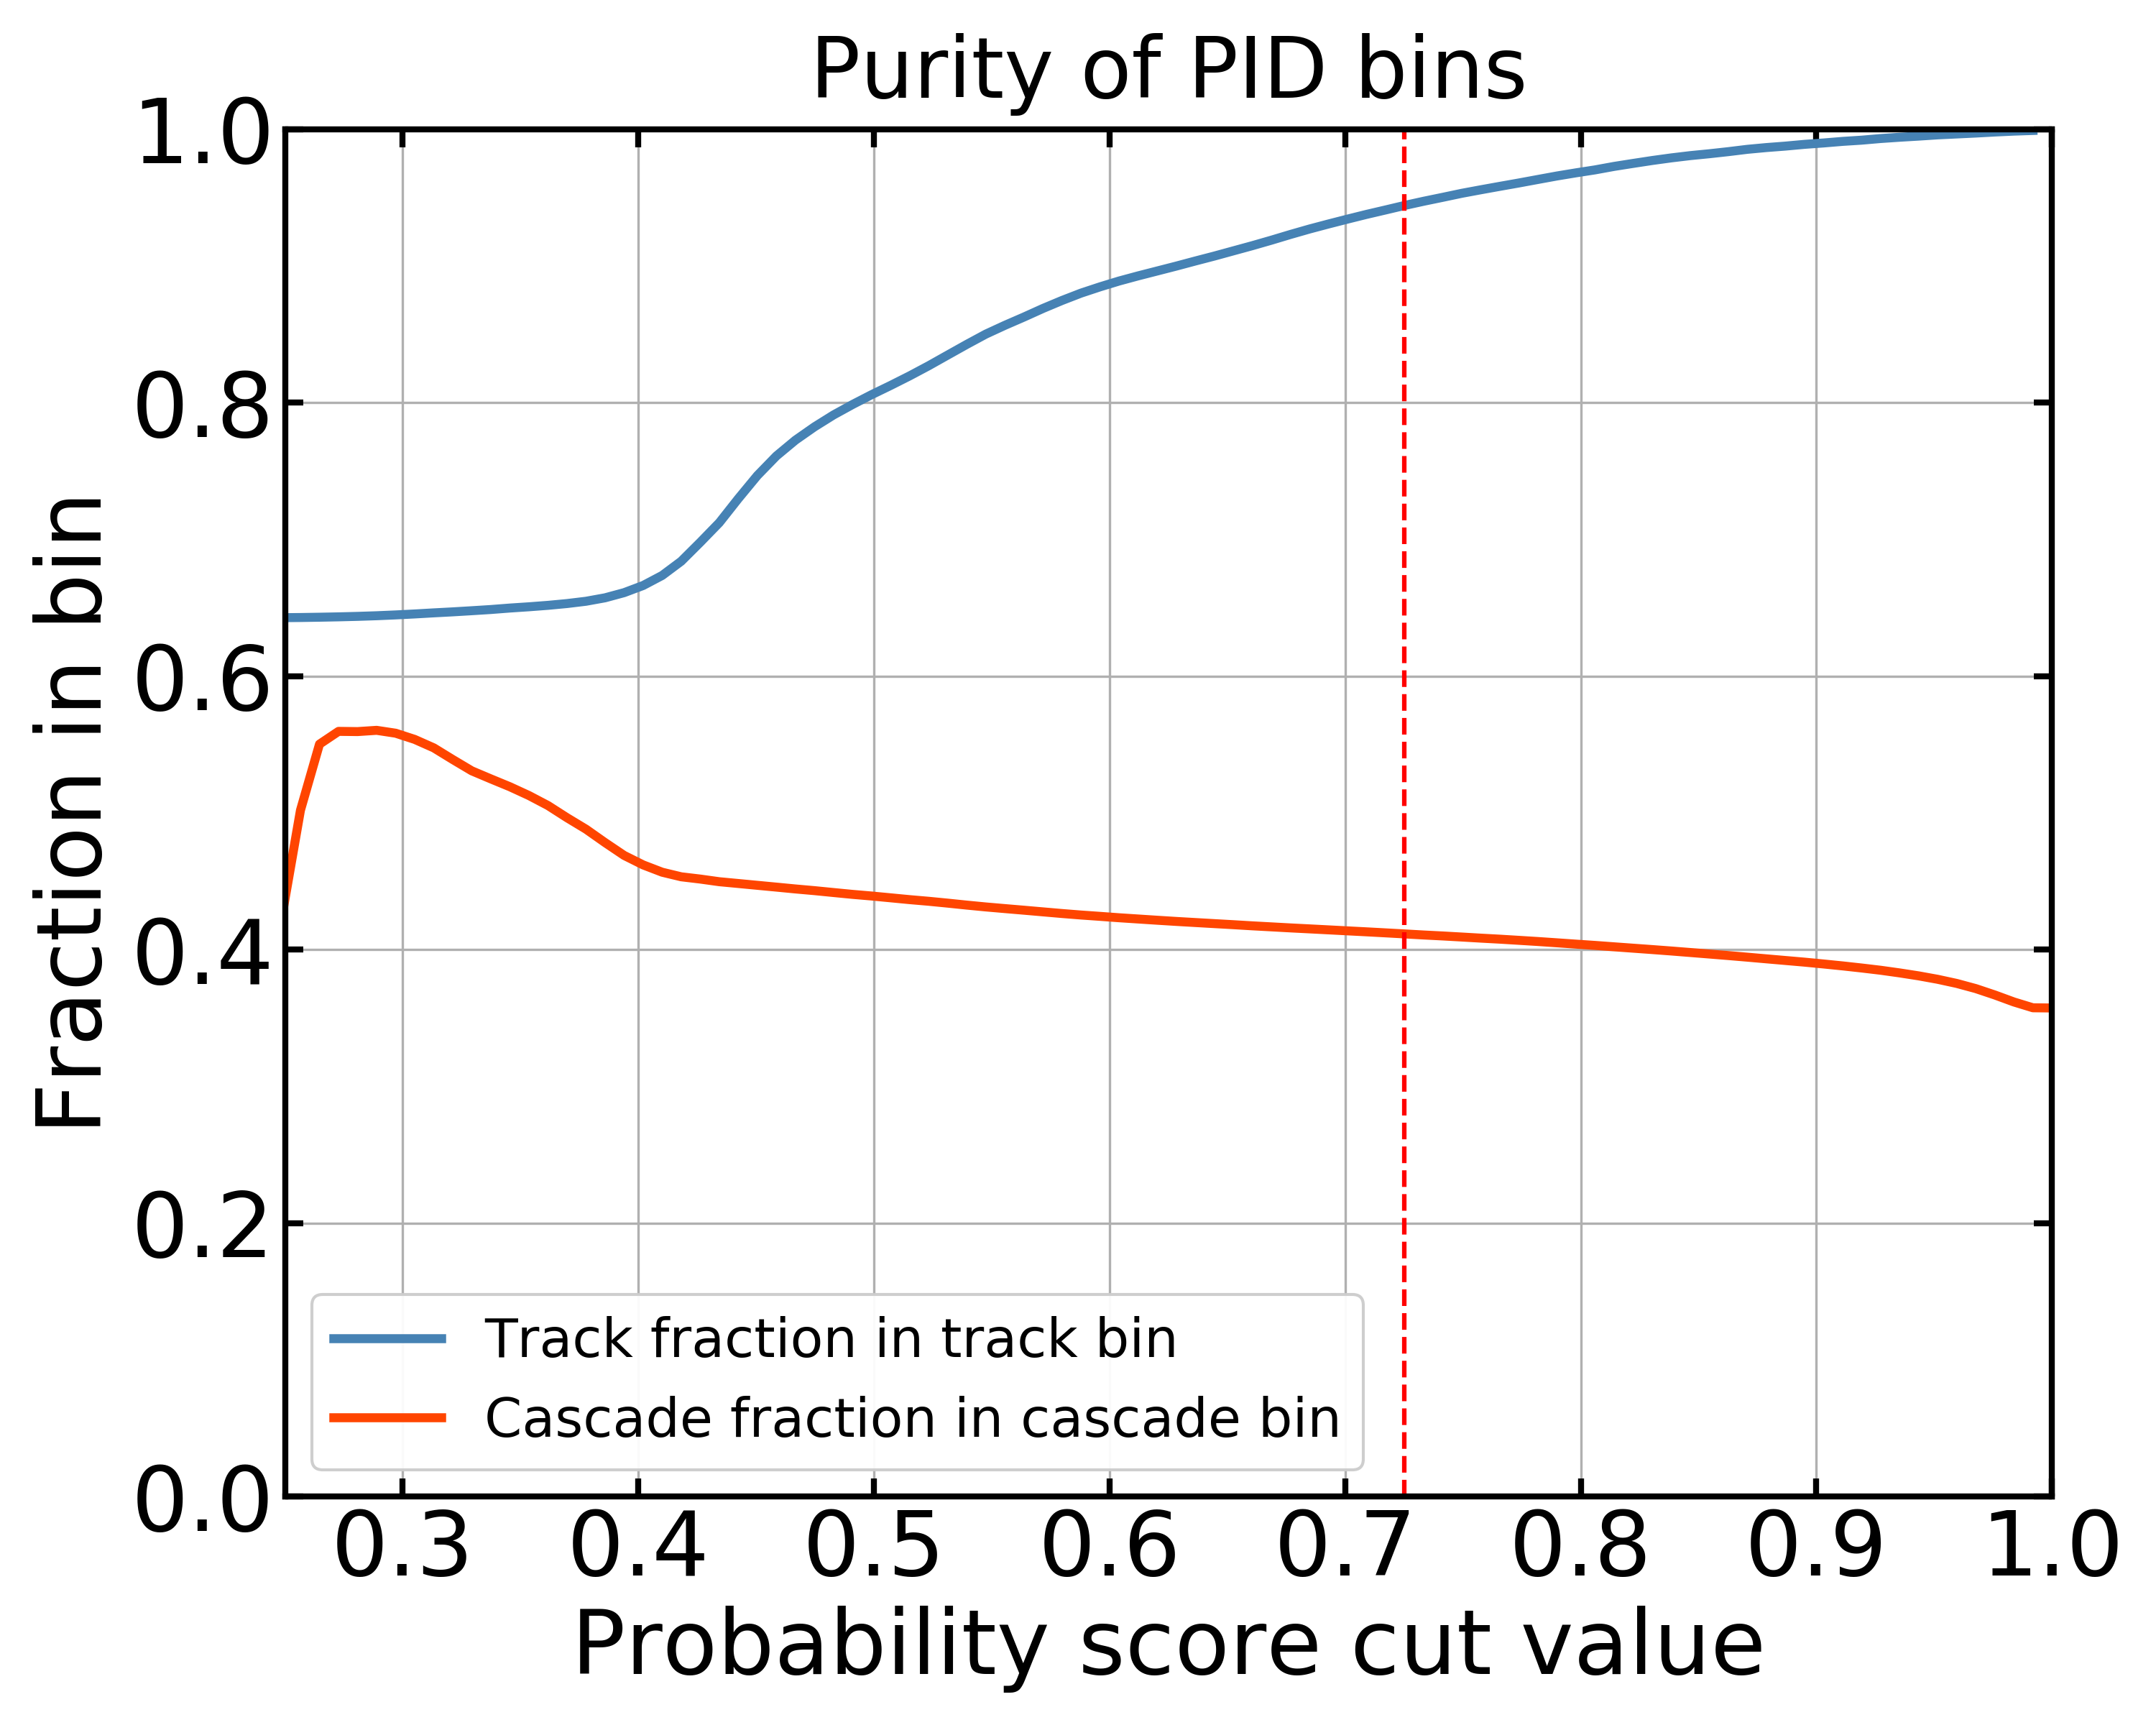
\includegraphics[width=0.49\linewidth]{figures/classifier_2_bin_contaminations.png}
    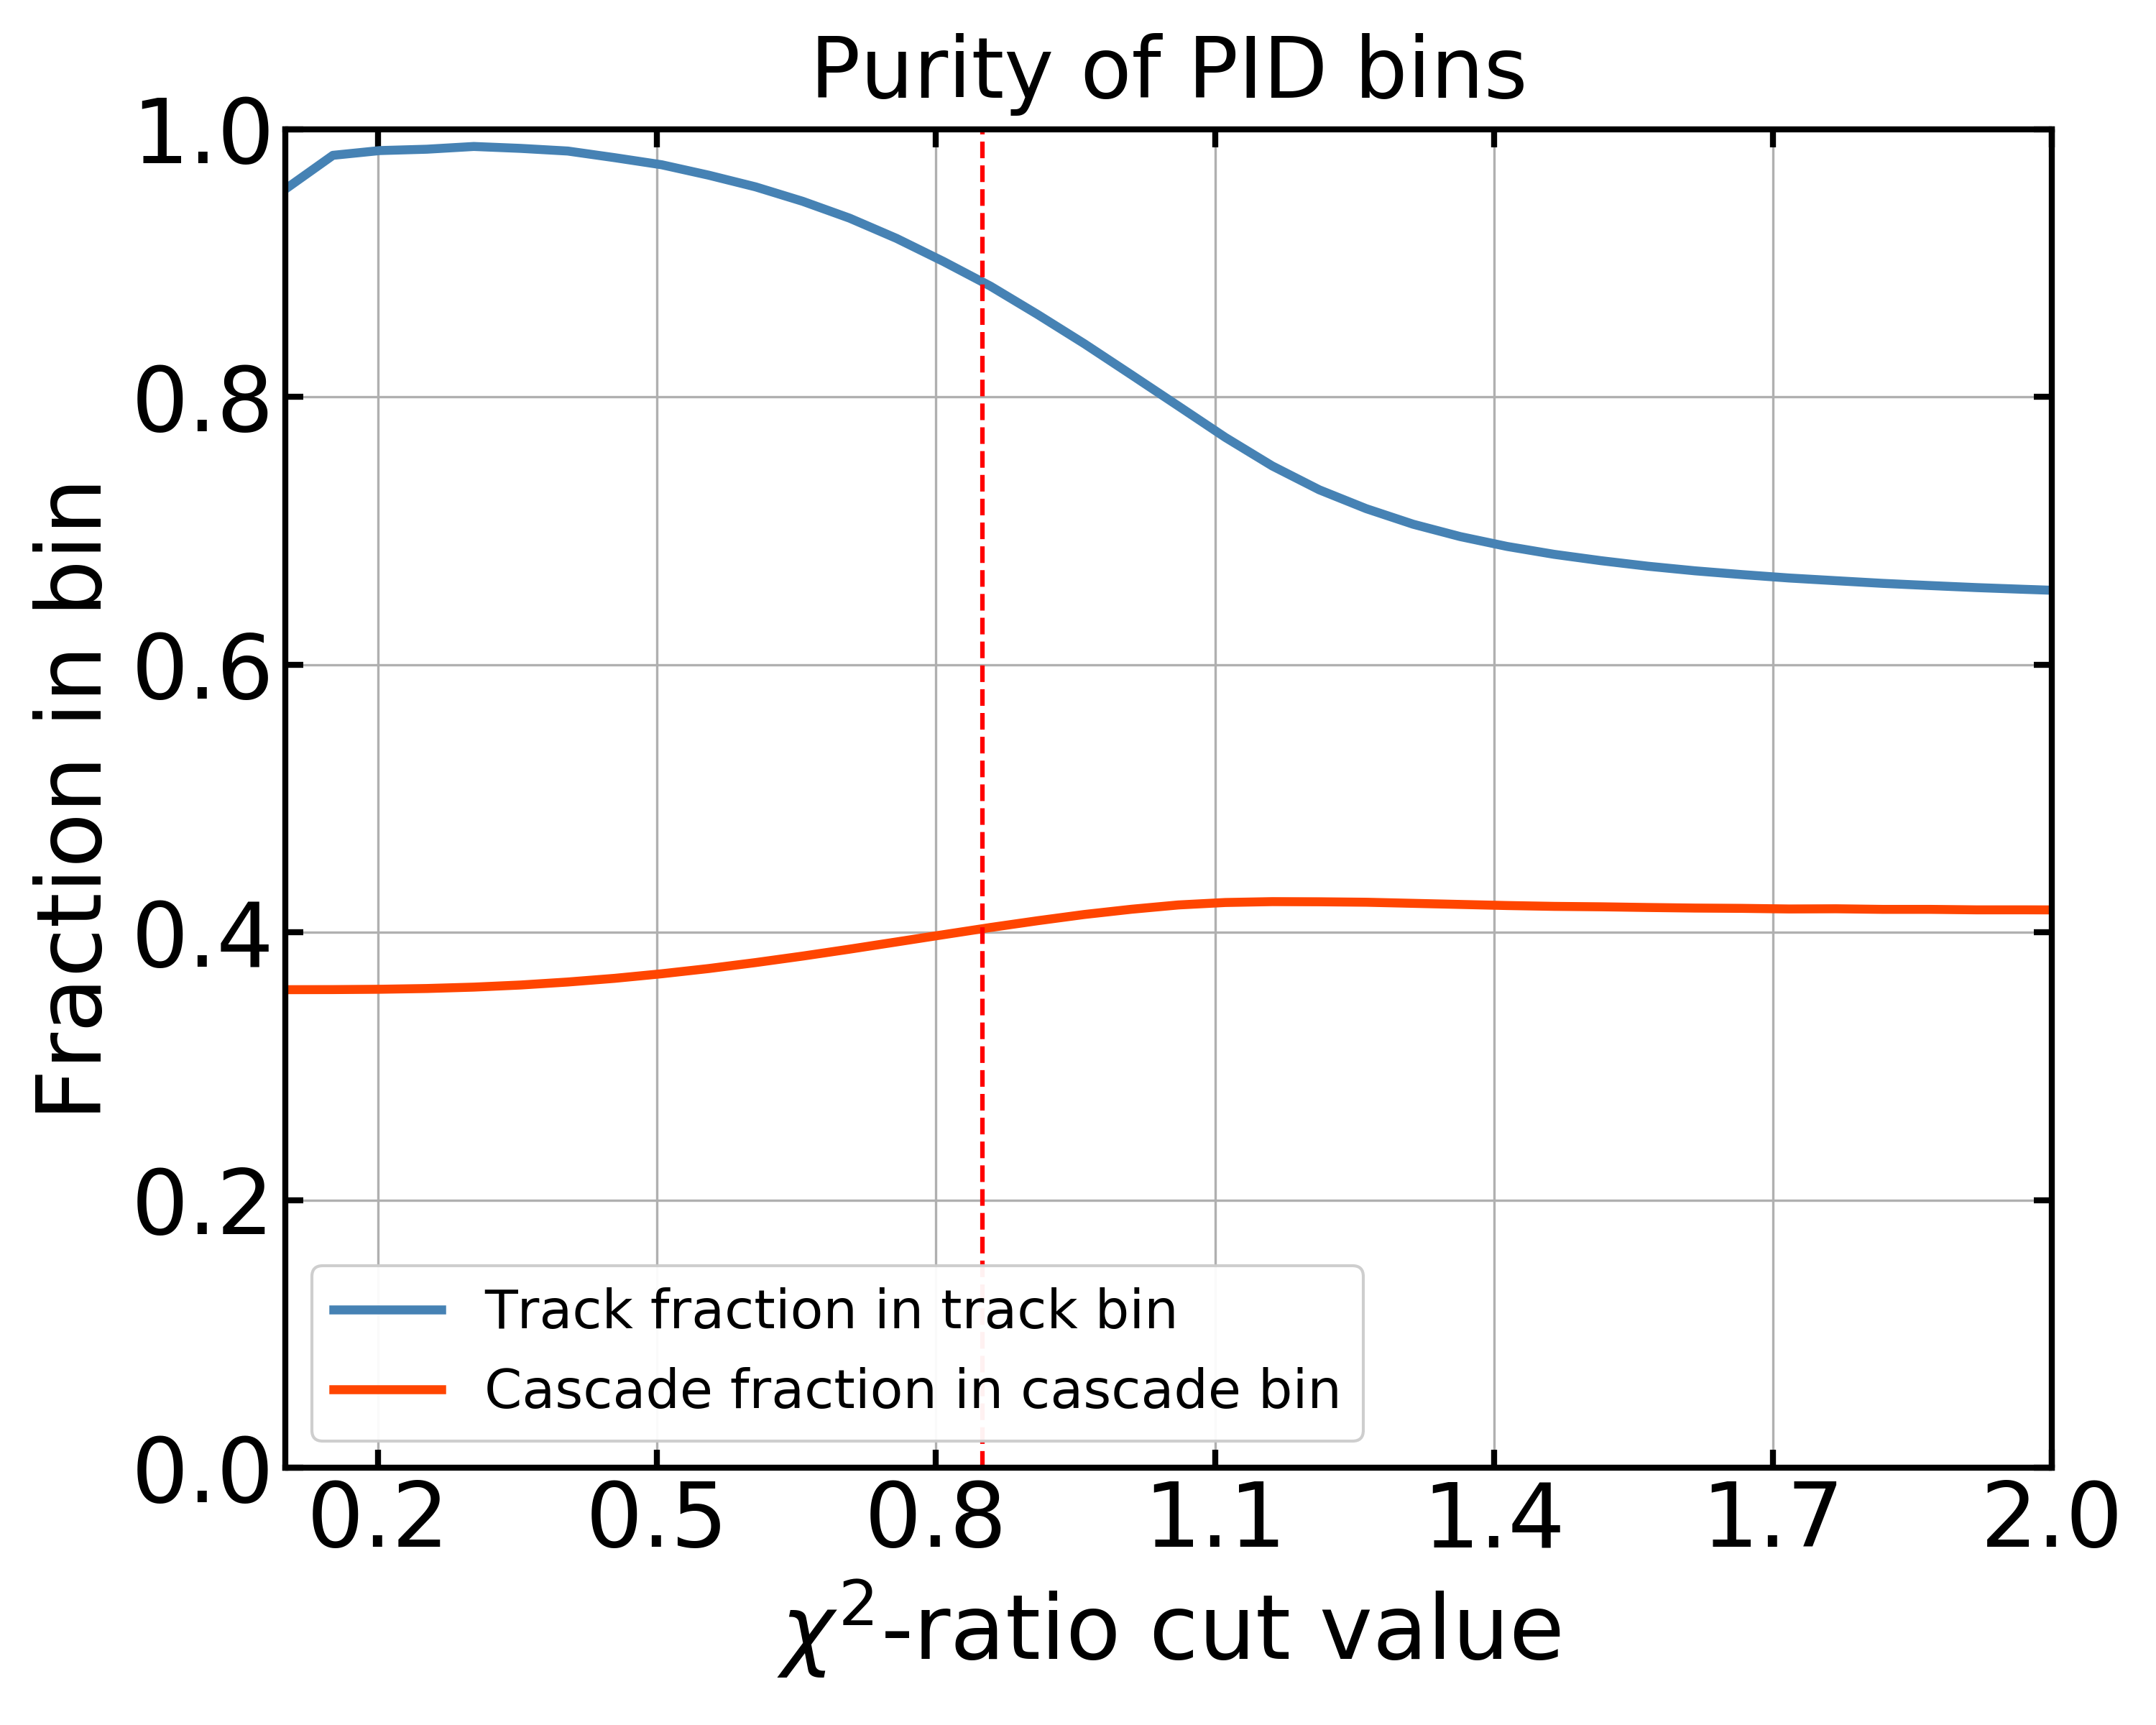
\includegraphics[width=0.49\linewidth]{figures/santa_2_bin_contaminations.png}
    \caption[Purity of the PID binning depending on PID cut value]
    {Purity of the PID binning depending on PID cut value for GBM probability (left) and  $\chi^2$-ratio (right). The chosen binning is indicated as a red, dashed line.}
    \label{fig:optimizing_two_bins_purity}
\end{figure}

To understand why the chosen binning results in the best sensitivities, the track/cascade purity of the bins is shown in Figure~\ref{fig:optimizing_two_bins_purity}.
The true track fraction in the track bin and the true cascade fraction in the cascade bin are shown.
It would be ideal if both were maximized, but a high purity of the track bin is more important since this is where we observe the primary disappearance signal.
For the GBM probability, the track purity increases with the PID cut, while the cascade purity decreases slightly.
Judging from this behavior it seems best to choose a large cut value which would lead to a very pure track sample.
\begin{figure}[h!]
    \centering
    \subfloat[probability score PID]{
    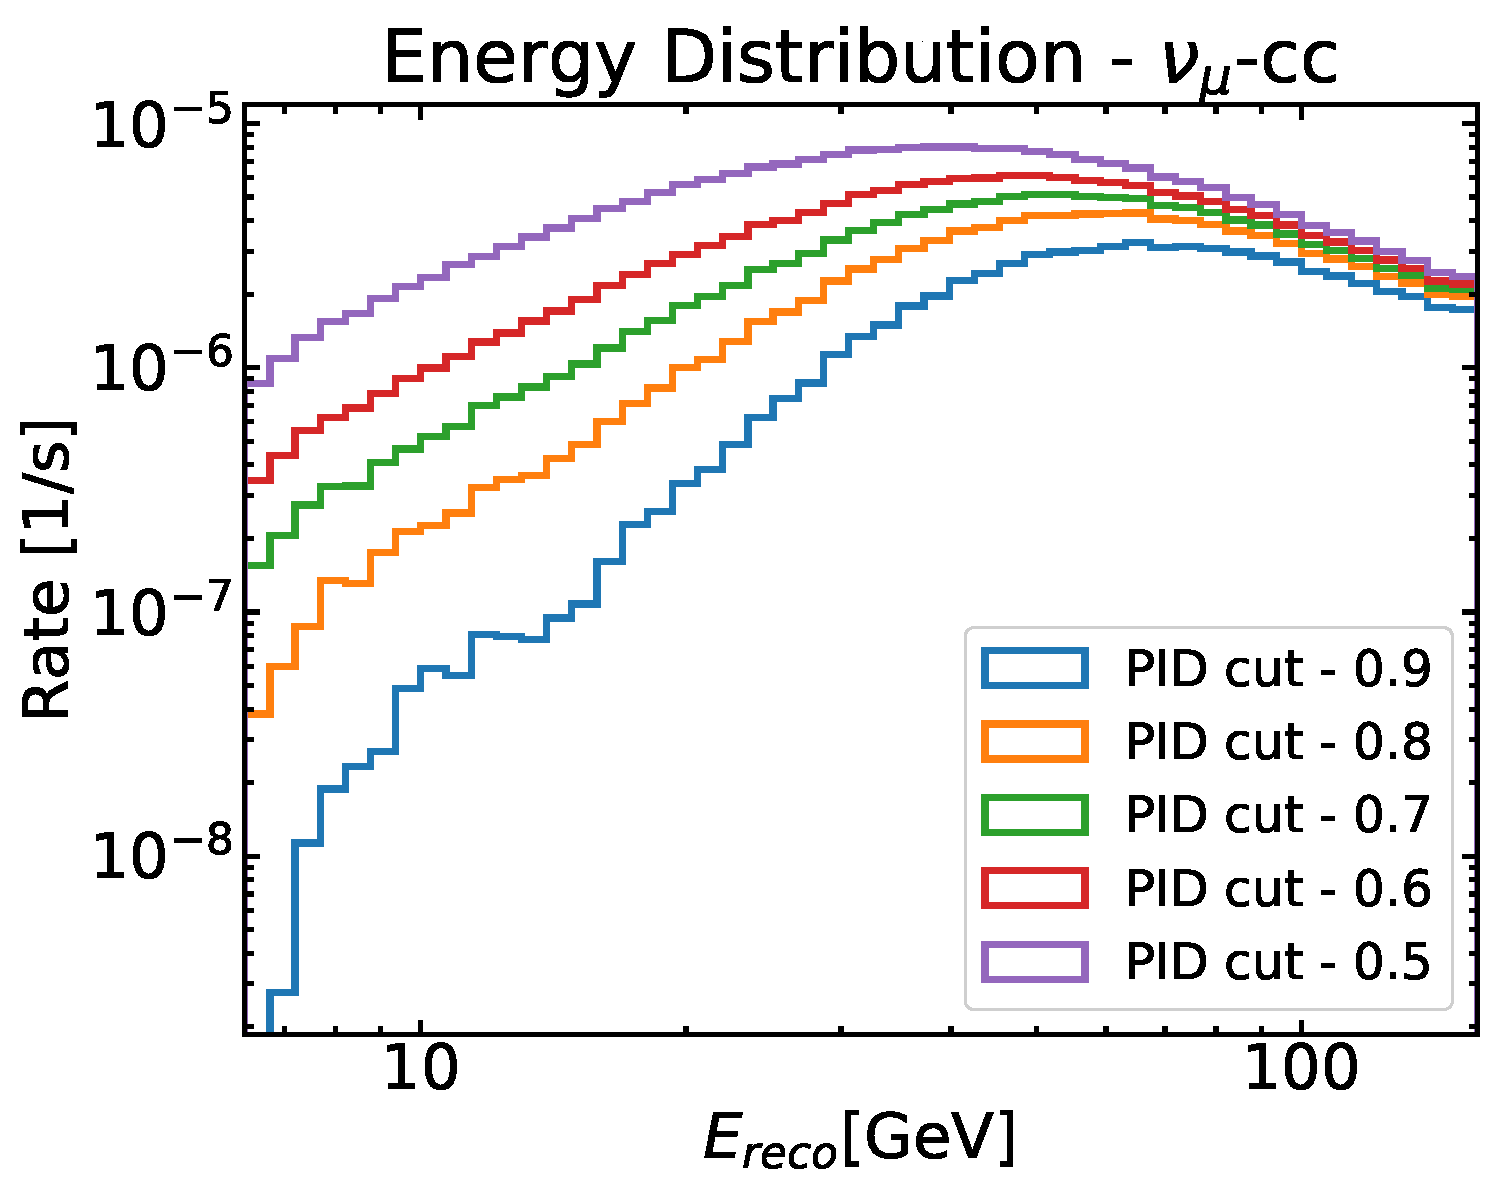
\includegraphics[width=0.48\linewidth]{figures/numu_cc_energy_distr_classifier_pid_cuts_logticks.pdf}
    }
    \subfloat[$\chi^2$-ratio PID]{
    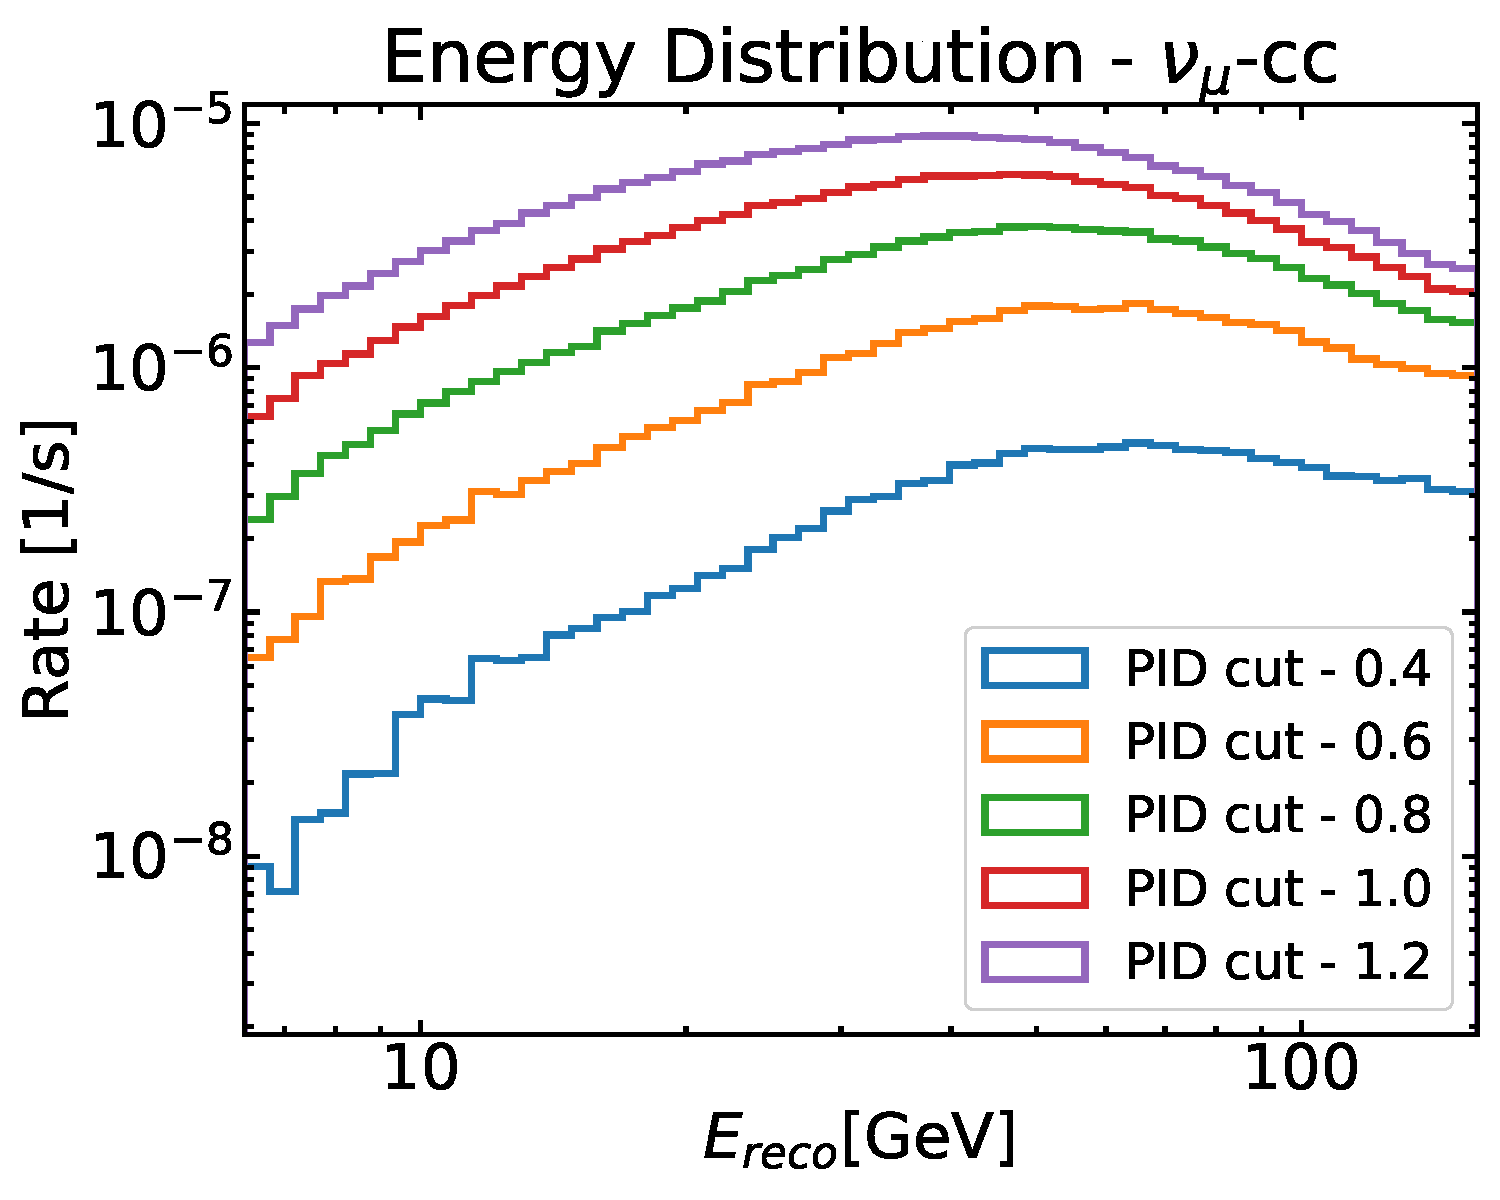
\includegraphics[width=0.48\linewidth]{figures/numu_cc_energy_distr_santa_pid_cuts_logticks.pdf}
    }
    \caption[Energy distribution of $\nu_\mu$-CC events in the track bin]{Energy distribution of $\nu_\mu$-CC events in the track bin cut on GBM probability (left) and on $\chi^2$-ratio (right).}
    \label{fig:energy_distribution_pid_bin}
\end{figure}
However, the left plot in Figure~\ref{fig:energy_distribution_pid_bin} shows that with the chosen GBM probability cut at 0.725 we maintain a reasonable event rate in the energy range of 20-40\,GeV, where the most dramatic oscillation effects are observed.
For larger cut values the rate in this energy region decreases strongly.
For the chosen cut value on the probability score, the resulting purities are 94.4\,\% track purity (track bin) and 41.2\,\% cascade purity (cascade bin).

The purity behavior for the cut on the $\chi^2$-ratio is reversed, due to the fact that low $\chi^2$-ratio values indicate tracks and high values indicate cascades.
The cascade purity is almost constant while the track purity decreases with increasing values of $\chi^2$-ratio.
This seems to indicate that a small PID cut value would be best, but comparing with the energy distributions for different cut values shown in the right plot of Figure~\ref{fig:energy_distribution_pid_bin}, we see that below a cut value of $\sim$0.8 the rate decreases strongly in the region of the oscillation signal.
For the chosen cut of 0.85 on the $\chi^2$-ratio PID we get 88.6\,\% track purity and 40.3\,\% cascade purity.

With these optimize cuts, we divide events into track-like or cascade-like samples.
The expected $E$ and $\cos\theta_z$ distributions for each sample are shown in Figure~\ref{fig:oscillation_effects_santa_2bin} and Figure~\ref{fig:oscillation_effects_gbm_2bin} for the $\chi^2$-ratio PID and the GBM probability PID, respectively.
\begin{figure}[h]
    \centering
    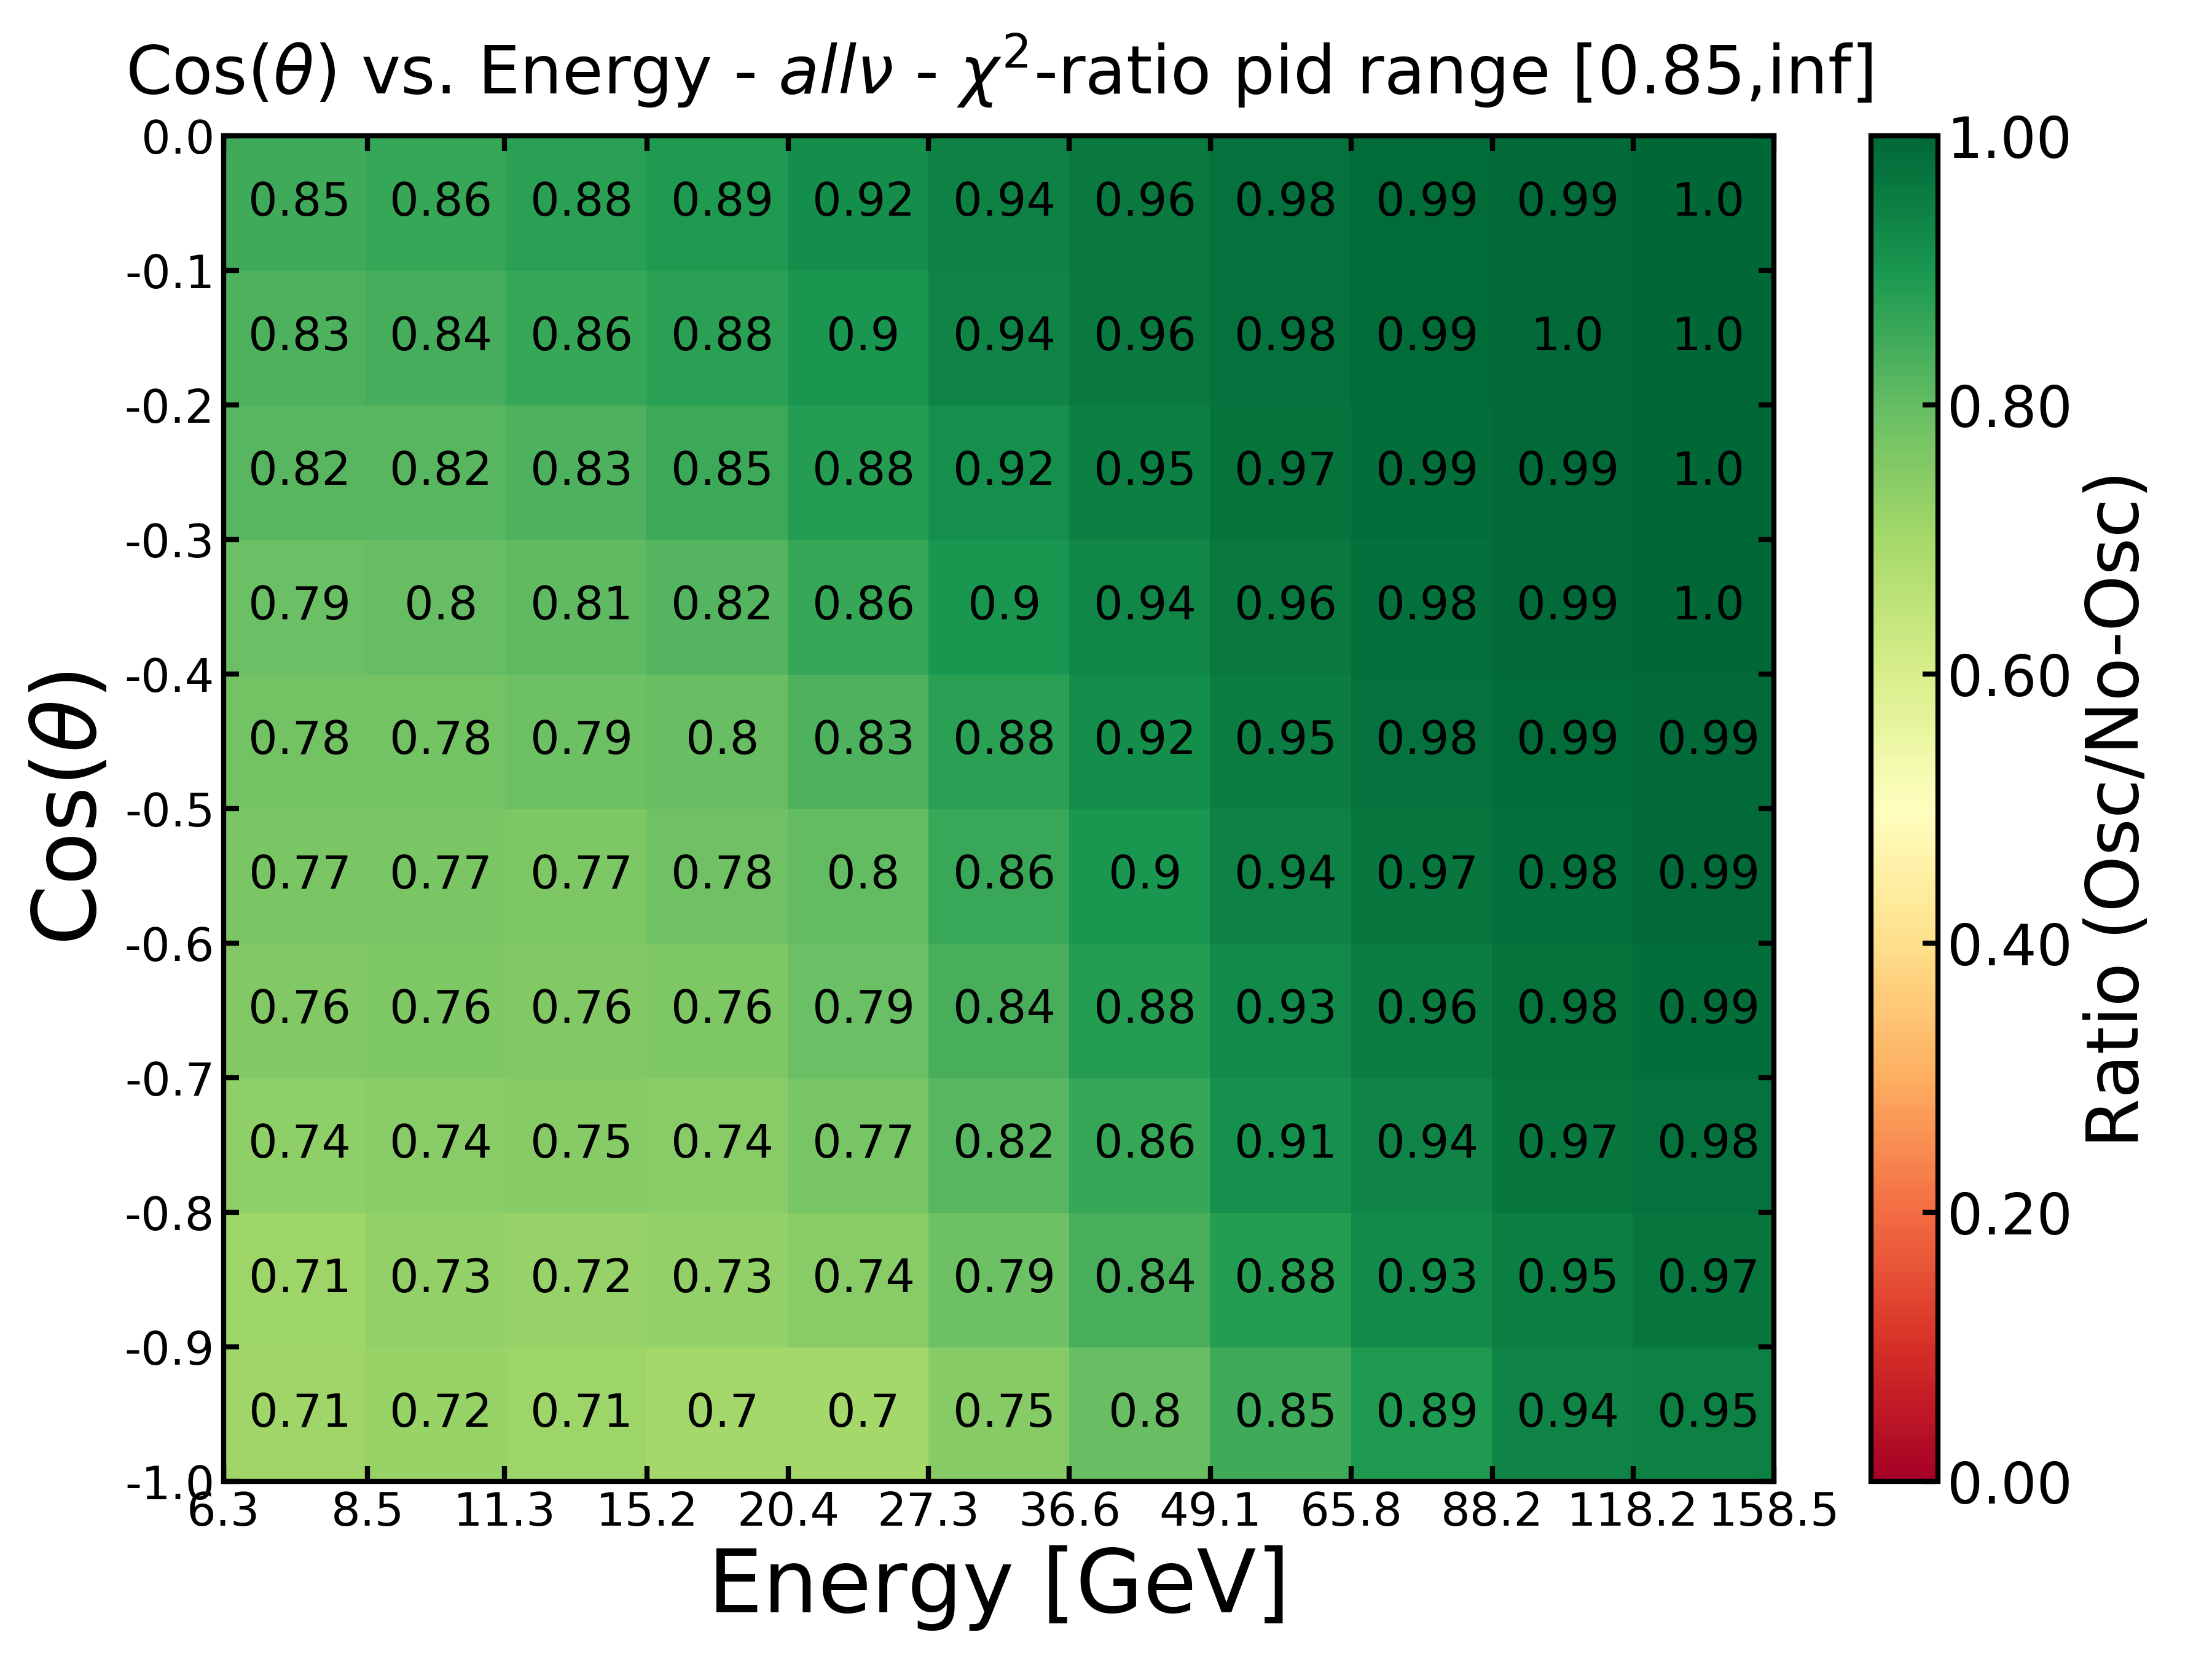
\includegraphics[width=0.49\linewidth]{figures/santa_cut_085_allnu_1_ratio_osc_noosc.png}
    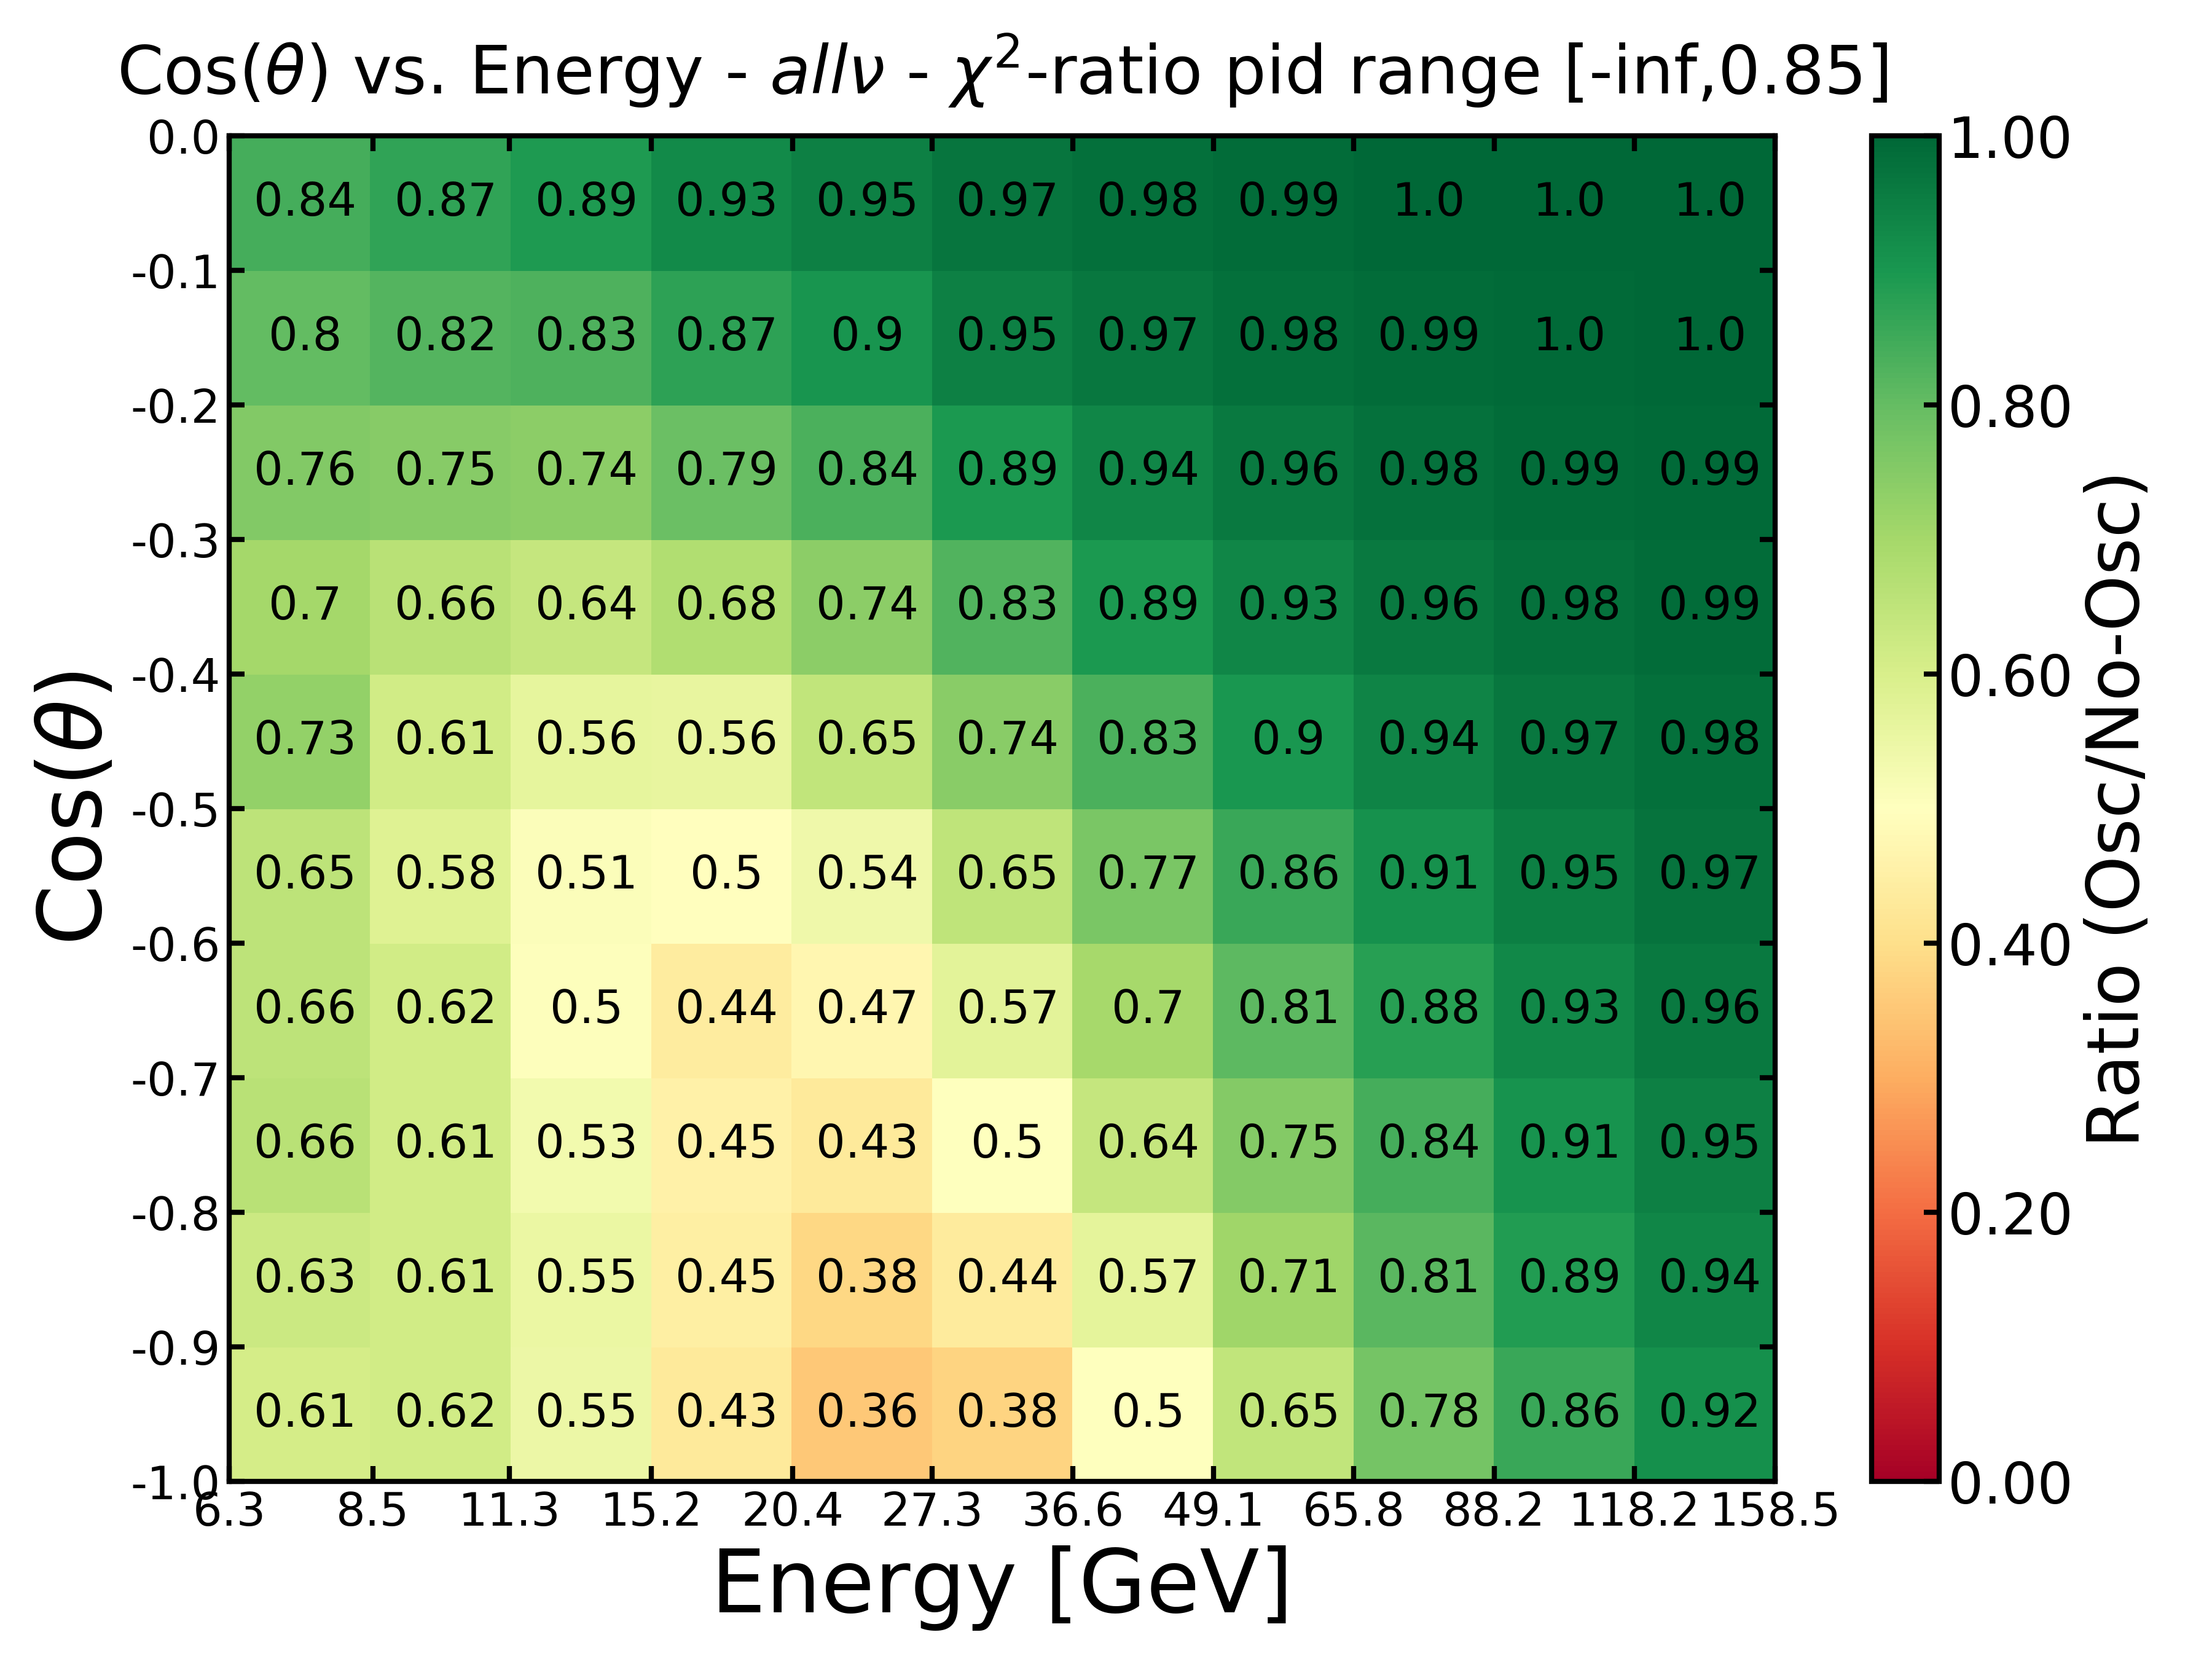
\includegraphics[width=0.49\linewidth]{figures/santa_cut_085_allnu_0_ratio_osc_noosc.png}
    \caption[Expected neutrino oscillation effects for two-bin case with $\chi^2\textrm{-ratio}$ PID]{Expected neutrino oscillation effects for two-bin case with $\chi^2\textrm{-ratio}$ PID. Shown is the ratio between un-oscillated and oscillated event rates for the cascade bin (left) and the track bin (right).}
    \label{fig:oscillation_effects_santa_2bin}
\end{figure}
\begin{figure}[h]
    \centering
    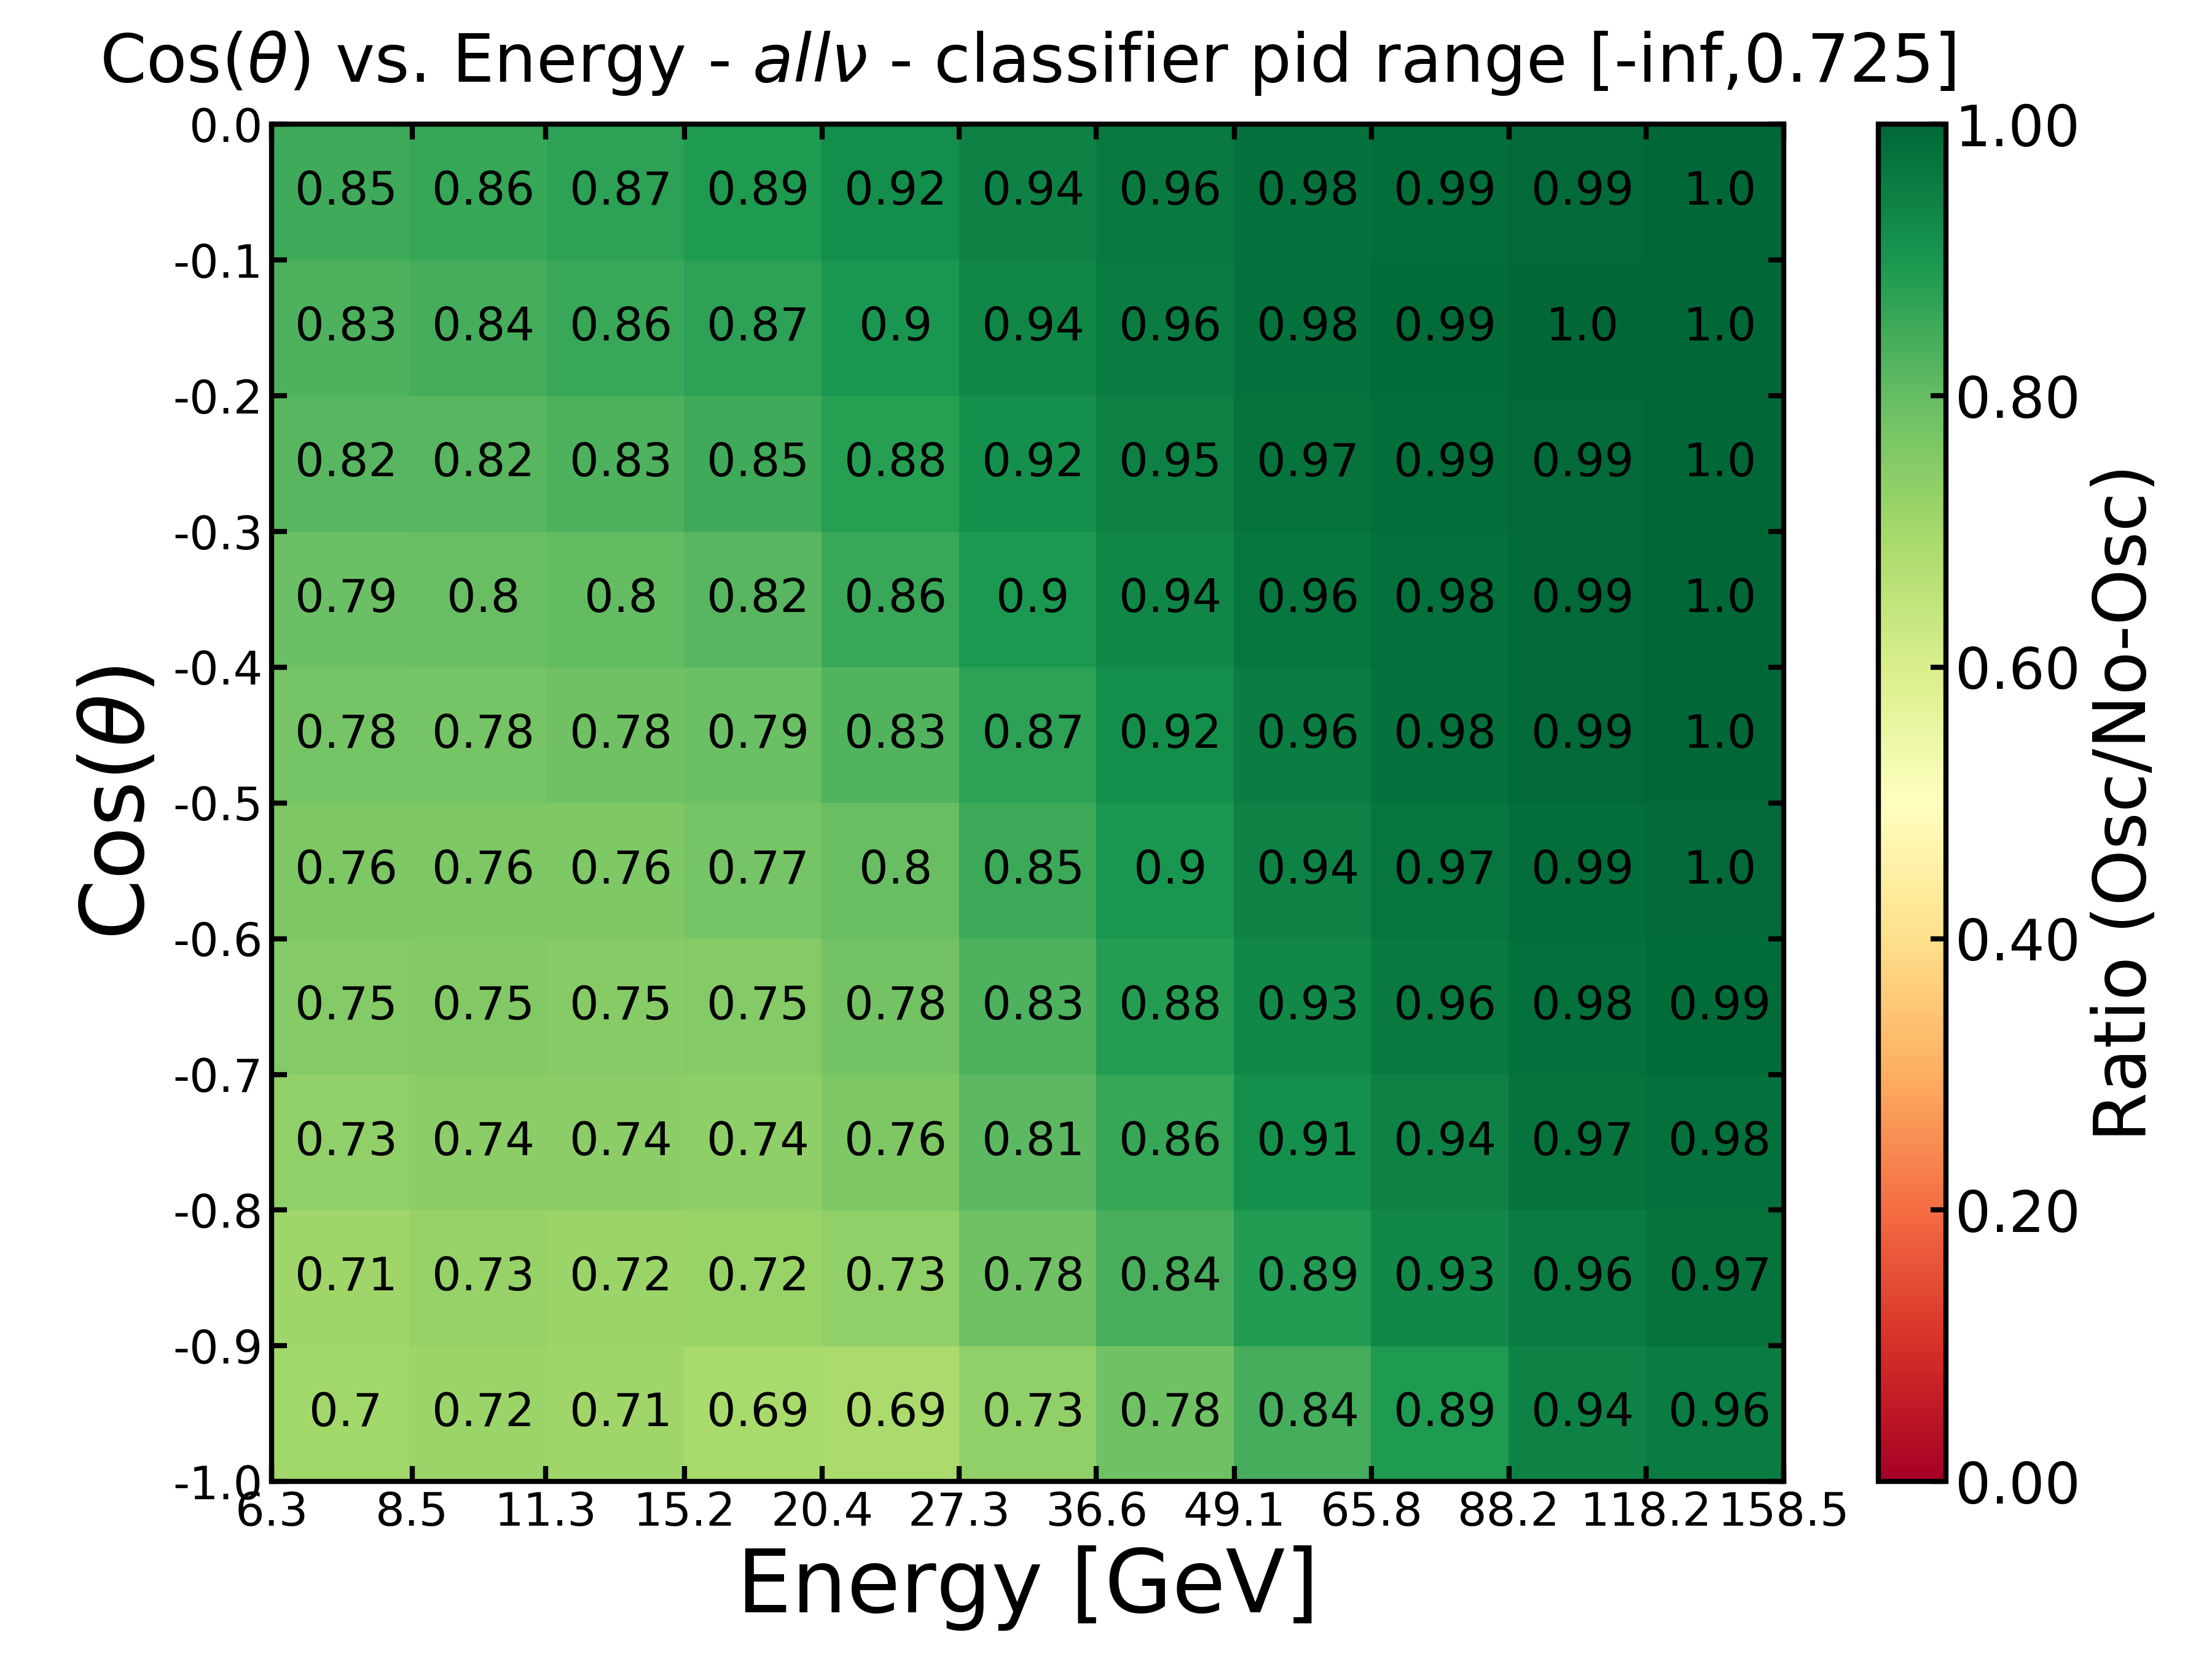
\includegraphics[width=0.49\linewidth]{figures/two_bin_cut_0725_allnu_0_ratio_osc_noosc.png}
    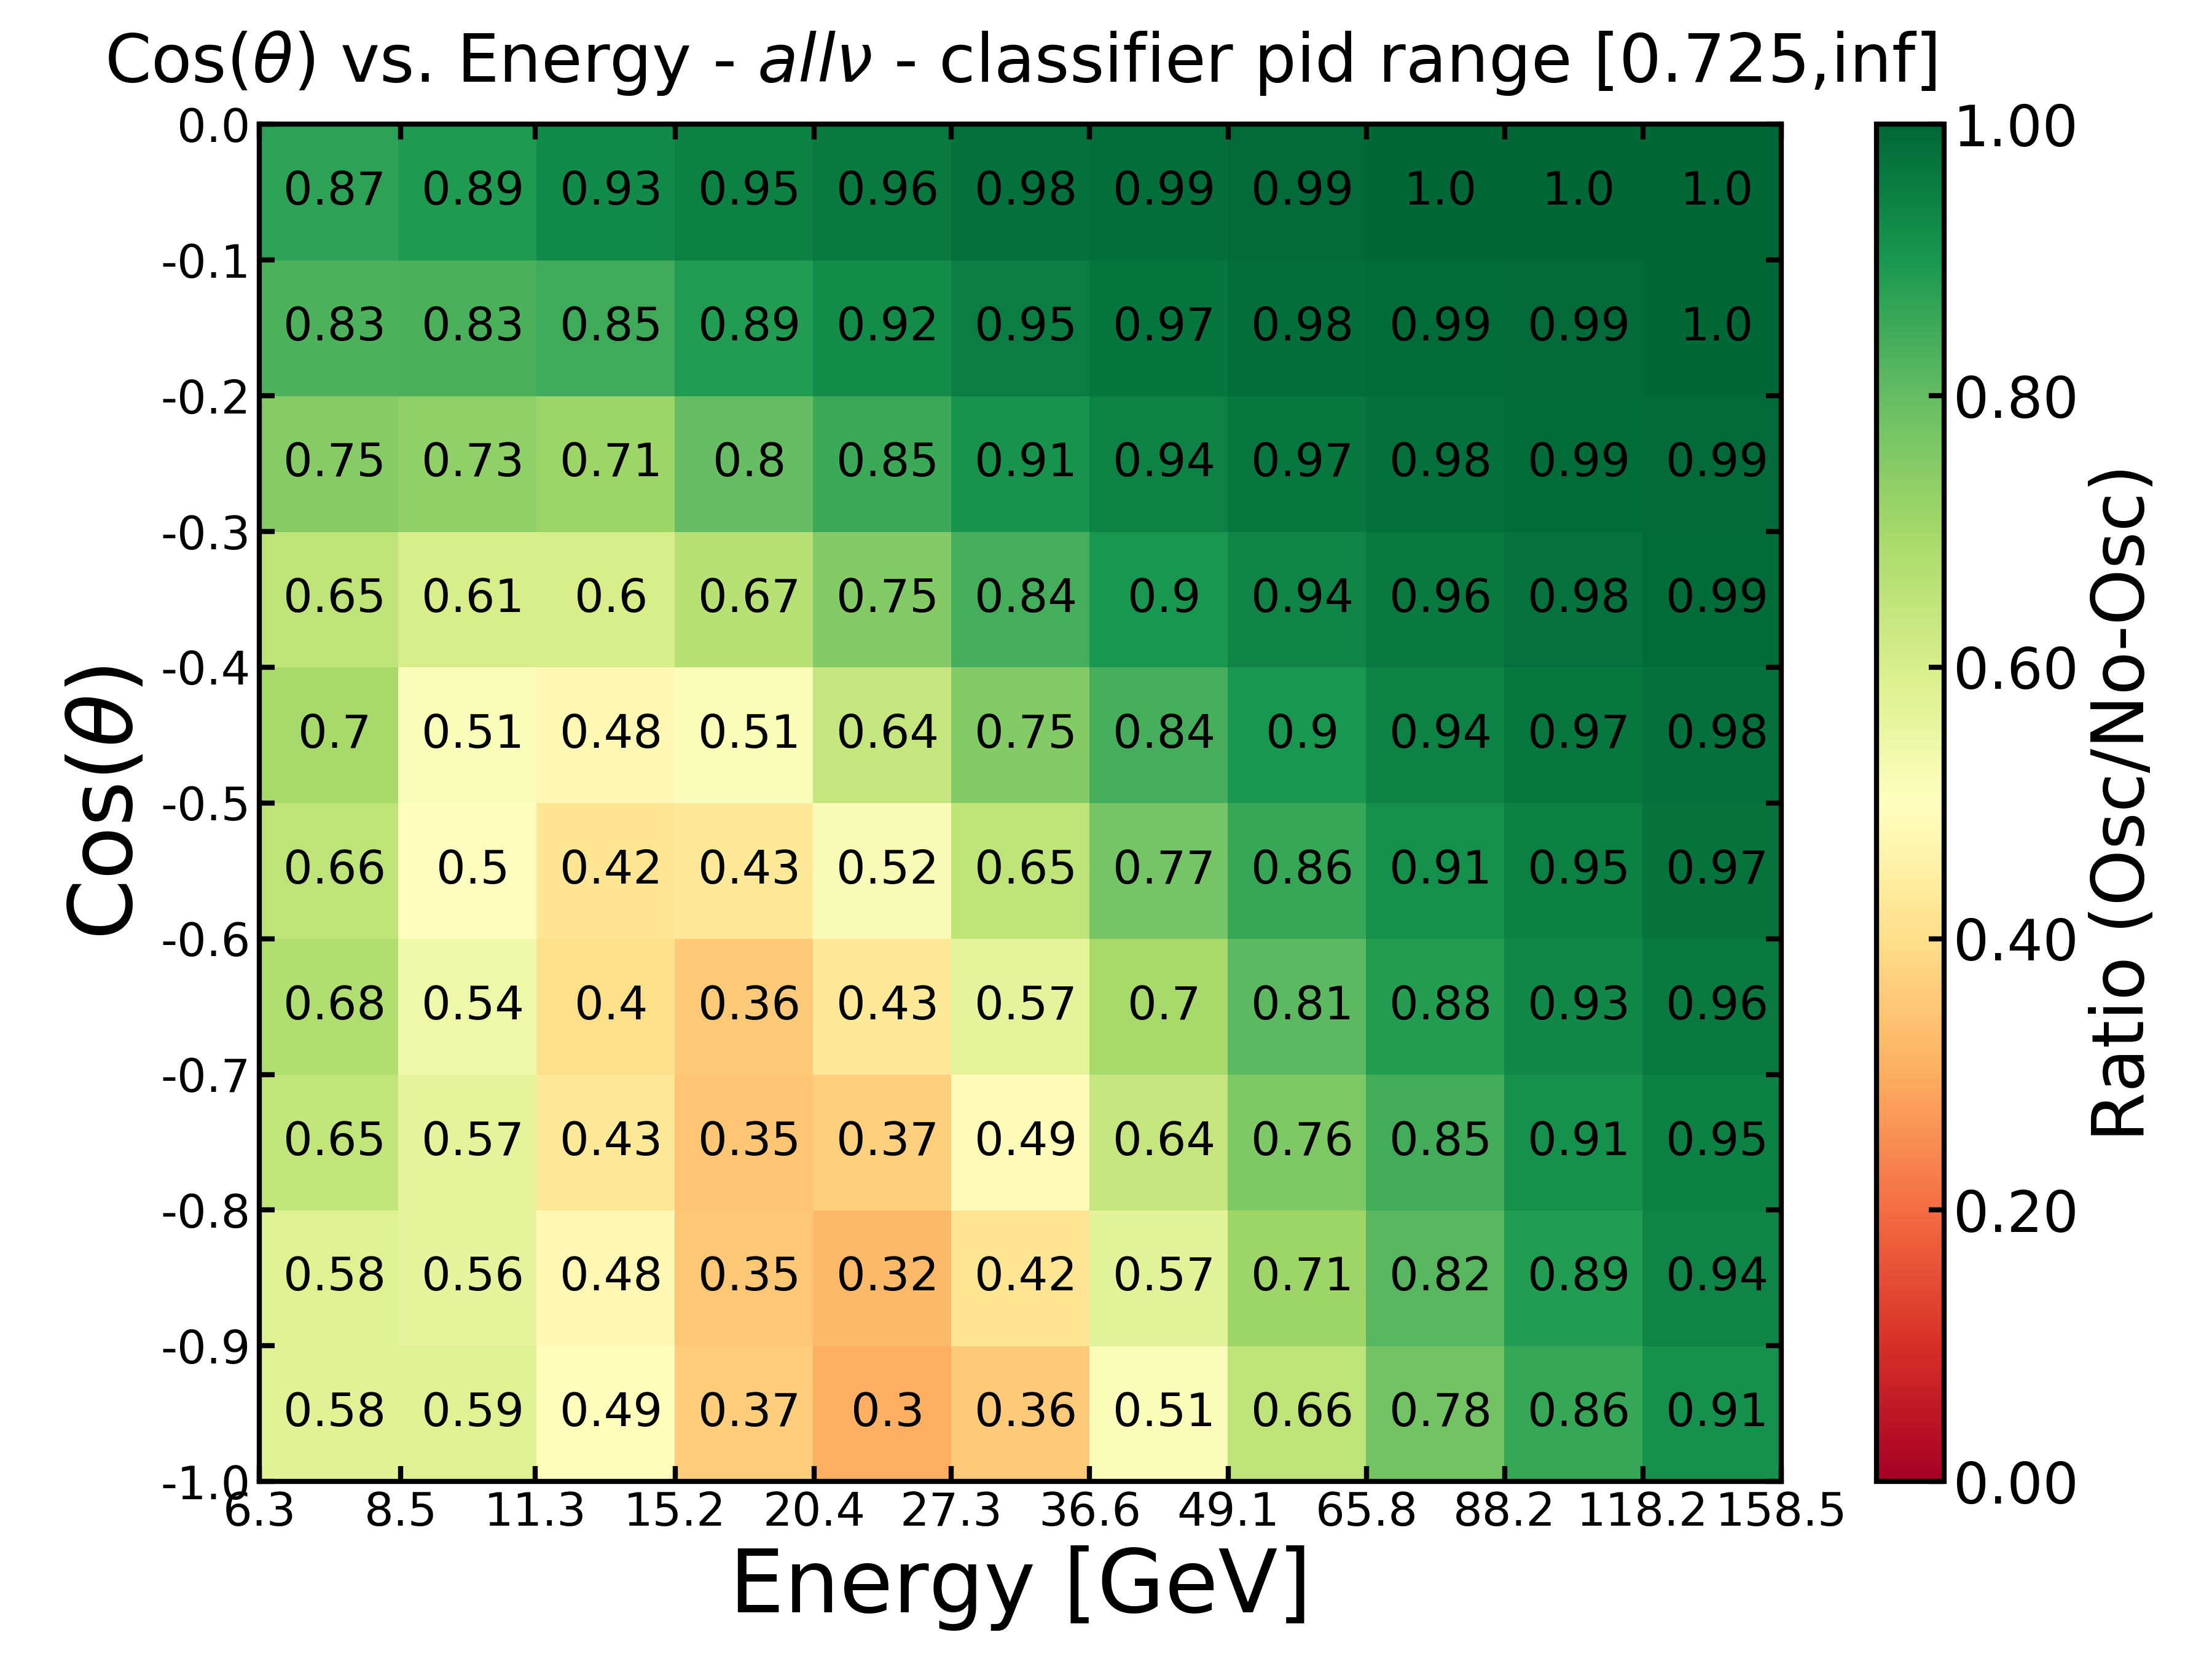
\includegraphics[width=0.49\linewidth]{figures/two_bin_cut_0725_allnu_1_ratio_osc_noosc.png}
    \caption[Expected neutrino oscillation effects for two-bin case with GBM probability]{Expected neutrino oscillation effects for two-bin case with GBM probability. Shown is the ratio between un-oscillated and oscillated event rates for the cascade bin (left) and the track bin (right).}
    \label{fig:oscillation_effects_gbm_2bin}
\end{figure}
The color scale indicates the ratio of the oscillated rate to the un-oscillated rate which shows the oscillation effect.
The oscillation signal is observed in the region where we expect it comparing with Figure~\ref{fig:muon_surv_prob}.
We also observe that the oscillation signal is stronger and more localized using the GBM probability PID and extends further into the region of horizontal events.
In Appendix~\ref{app:event_distributions} all the binned event rates are shown for the un-oscillated flux and the oscillated flux.

We also investigate the sensitivity that can be achieved using three PID bins.
The performance of the individual three-bin studies is visualized in Figure~\ref{fig:optimizing_three_bins}, where small uncertainties are dark blue.
\begin{figure}[h]
    \centering
    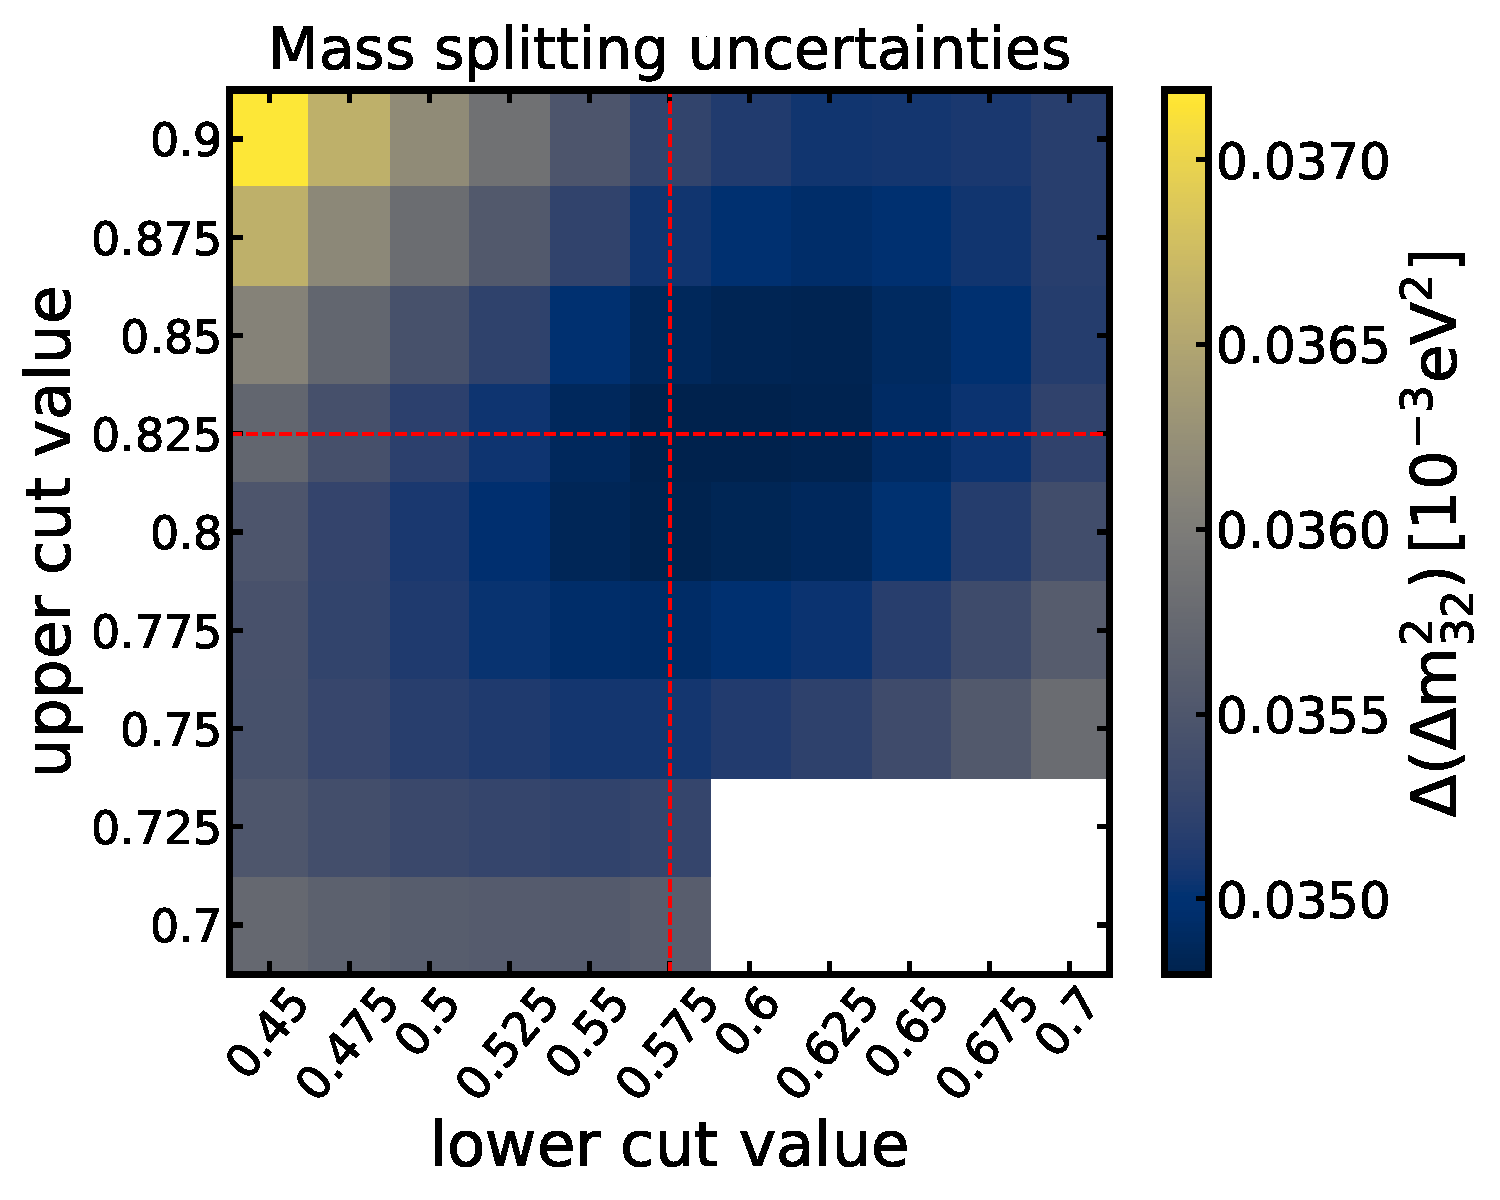
\includegraphics[width=0.49\linewidth]{figures/three_bin_optimization_mass_splitting_2dhist_cividis_cut_x.pdf}
    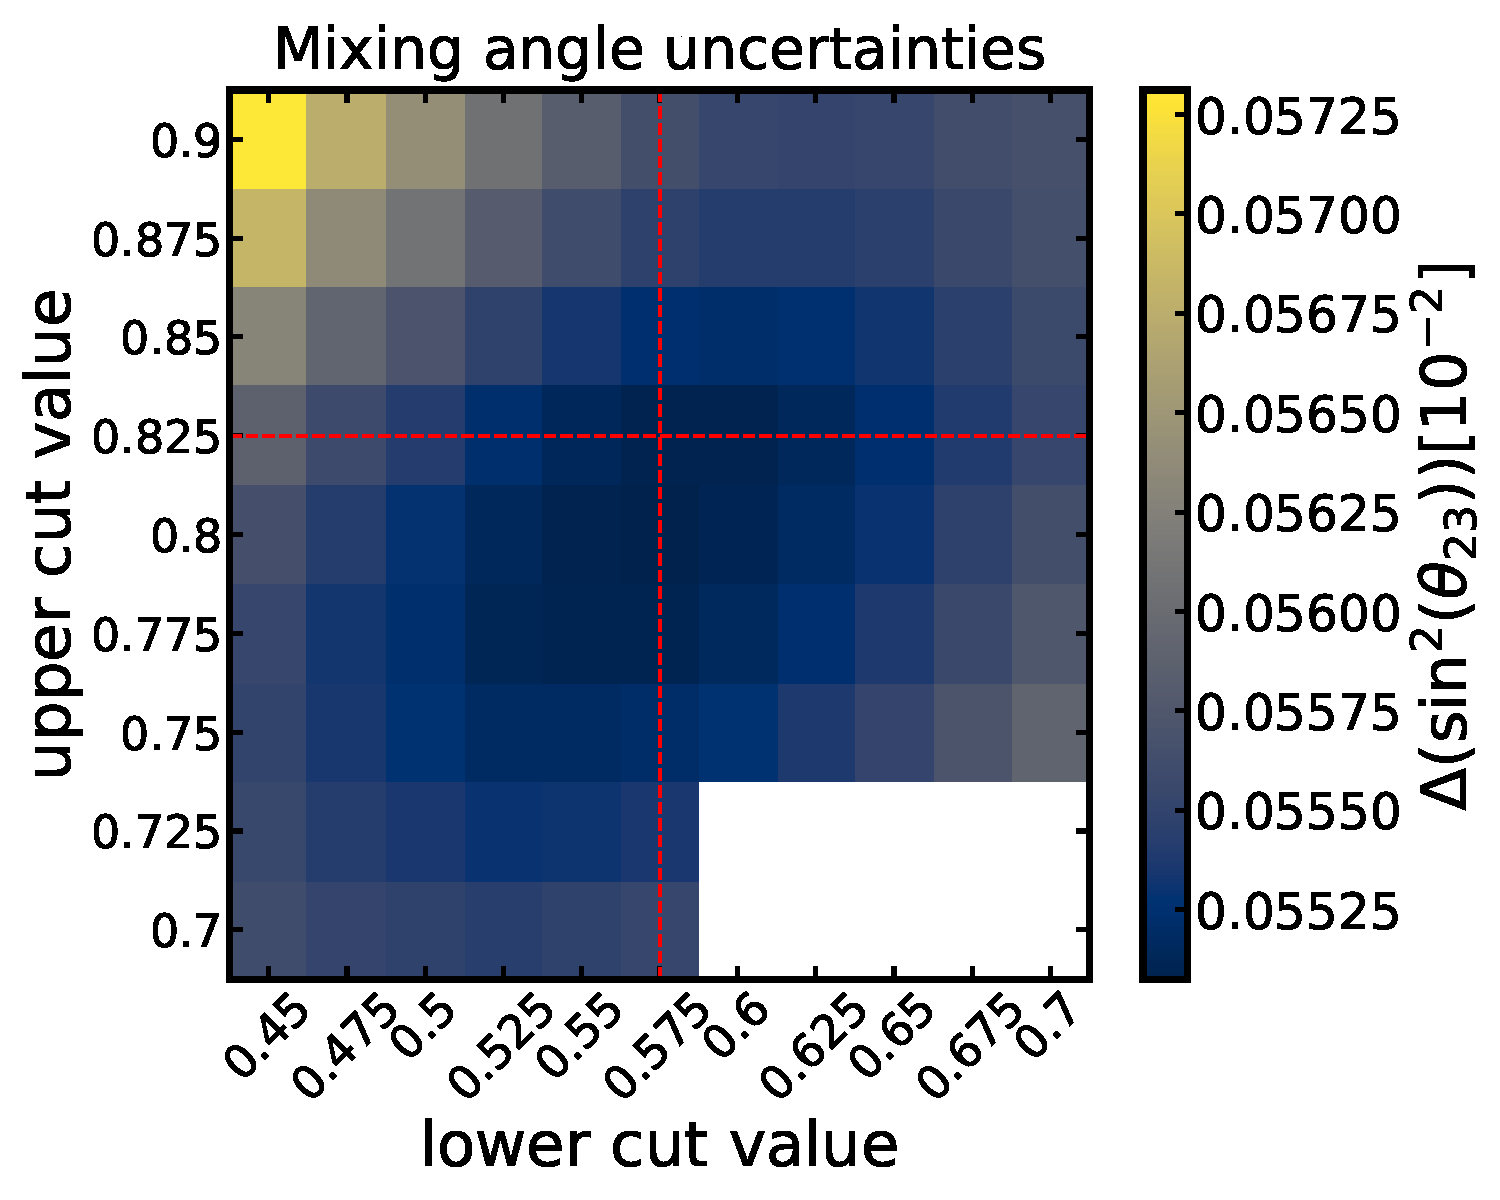
\includegraphics[width=0.49\linewidth]{figures/three_bin_optimization_mixing_angle_2dhist_cividis_cut_x.pdf}
    \caption[Sensitivity results of the three-bin PID cut optimization]{Sensitivity results of the three-bin PID cut optimization for the GBM probability. The optimal cut values are indicated as red, dashed lines. $\Delta(\Delta \mathrm{m}^{2}_{32})$ (left) and $\Delta(\sin^{2}(\theta_{23}))$ (right) are the sizes of the $68$\,\% C.L. for mixing angle and mass splitting, respectively.}
    \label{fig:optimizing_three_bins}
\end{figure}
There is a region where several cut combinations perform similarly good.
The best result with three bins is found for cut values 0.575 and 0.825, resulting in 97.6\,\% track purity (track bin), 77.0\,\% track purity (intermediate bin) and 43.7\,\% cascade purity (cascade bin).

Similar to how it was done for the two-bin cases, we apply these optimized cuts to divide the events into a track-like, a cascade-like, and a mixed sample.
We investigate the observed oscillation effects by taking the ratio of the oscillated rate to the un-oscillated rate as shown in Figure~\ref{fig:oscillation_effects_gbm_3bin}.
In the intermediate bin we see a weak oscillation effect, while in the track bin the effect is much stronger than in Figure~\ref{fig:oscillation_effects_santa_2bin}.
Additionally, the strength of the signal is larger than in Figure~\ref{fig:oscillation_effects_santa_2bin} and Figure~\ref{fig:oscillation_effects_gbm_2bin}.
The binned event rates for the un-oscillated flux and the oscillated flux are shown in Appendix~\ref{app:event_distributions}.

\begin{figure}[h]
    \centering
    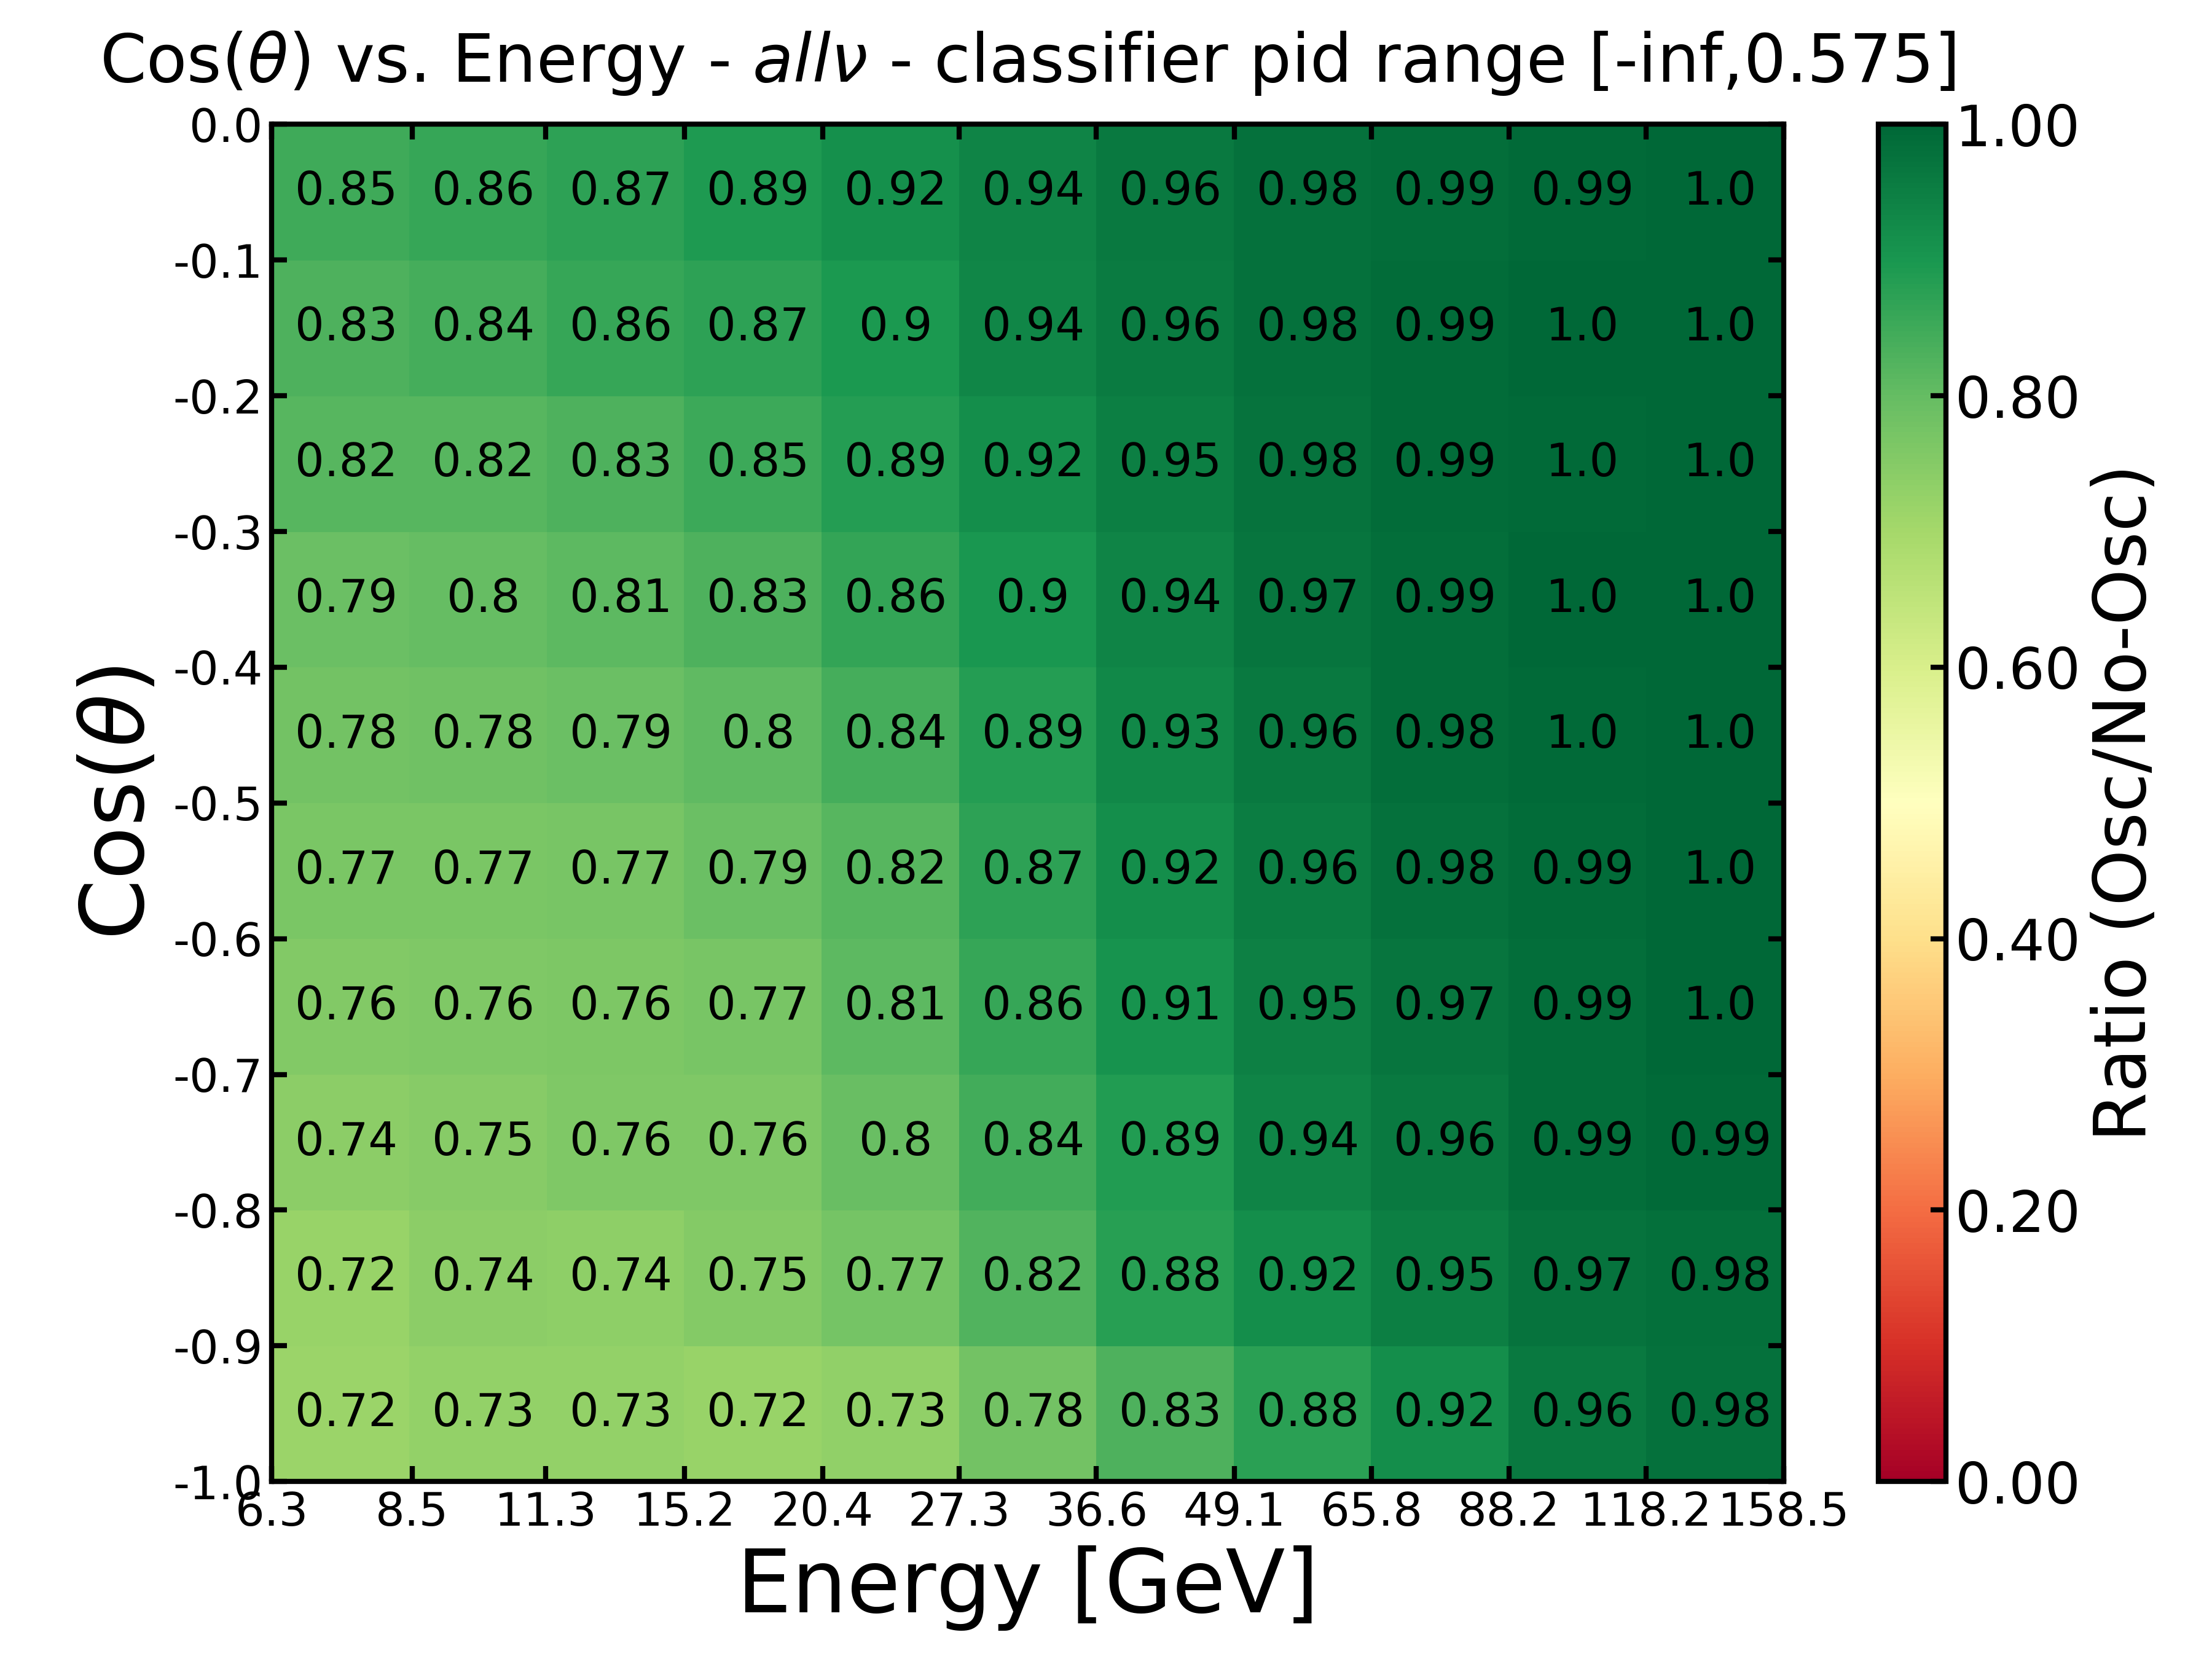
\includegraphics[width=0.49\linewidth]{figures/three_bin_cut_0575_0825_allnu_0_ratio_osc_noosc.png}
    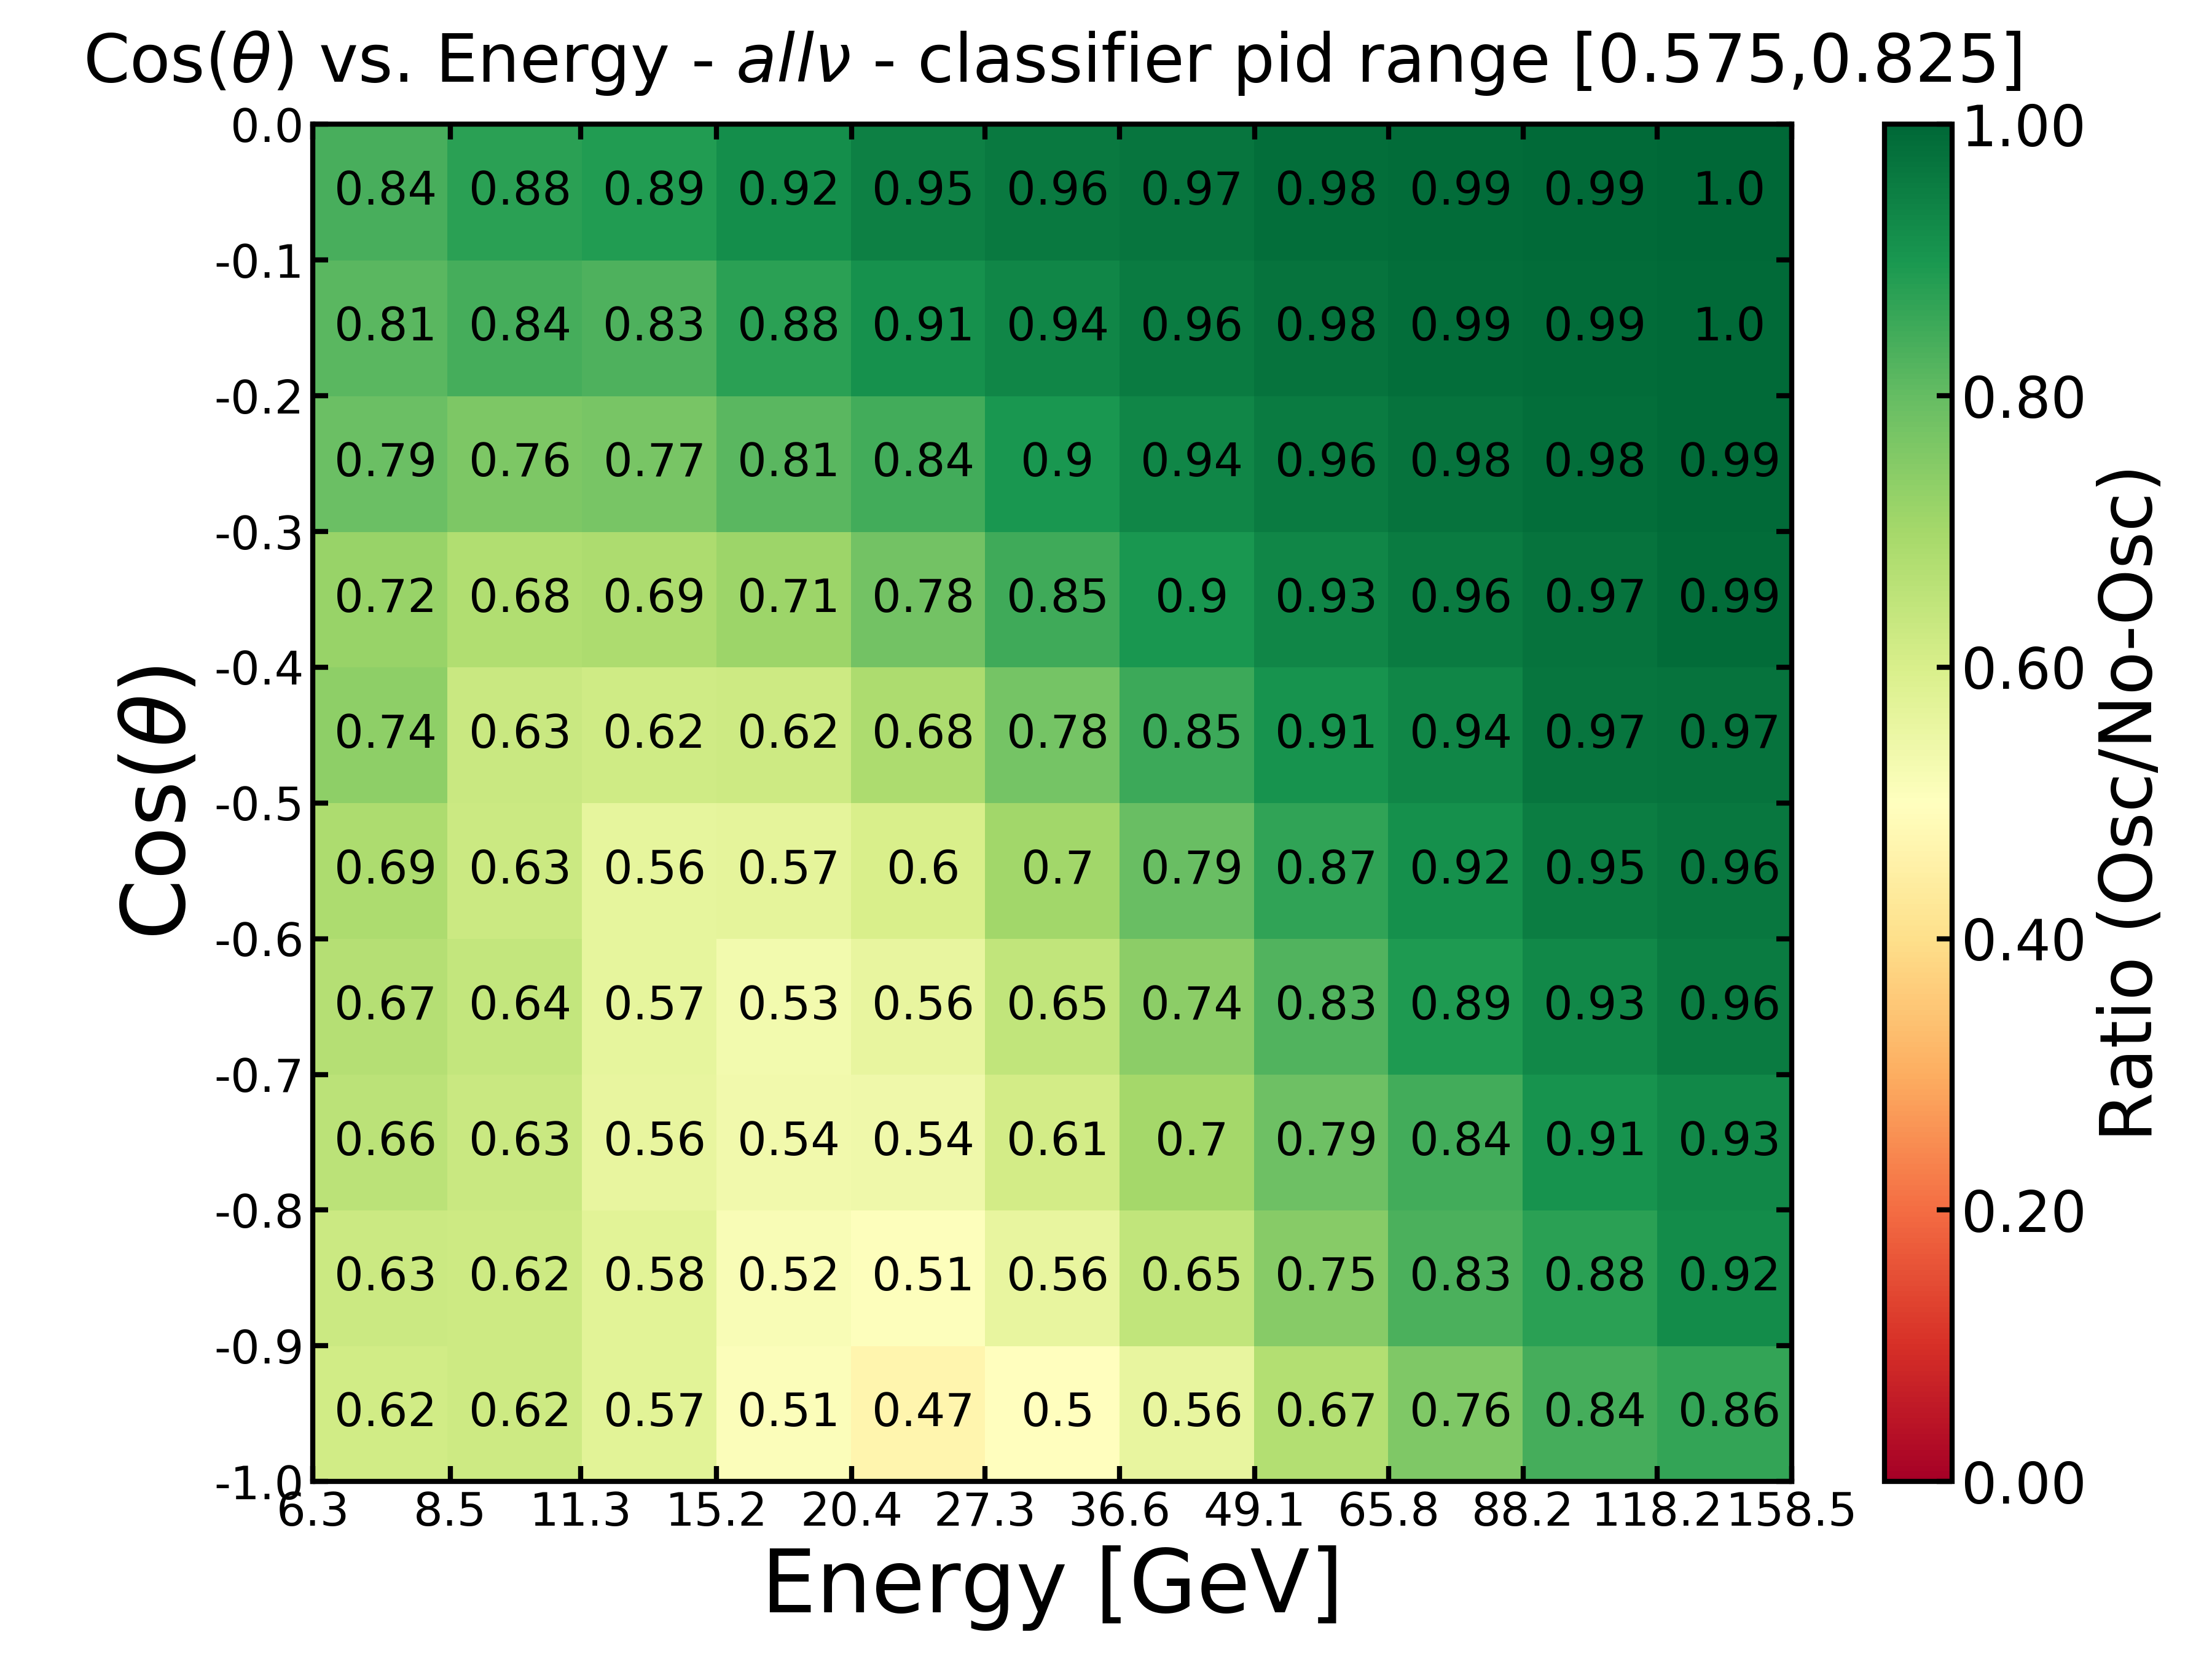
\includegraphics[width=0.49\linewidth]{figures/three_bin_cut_0575_0825_allnu_1_ratio_osc_noosc.png}
    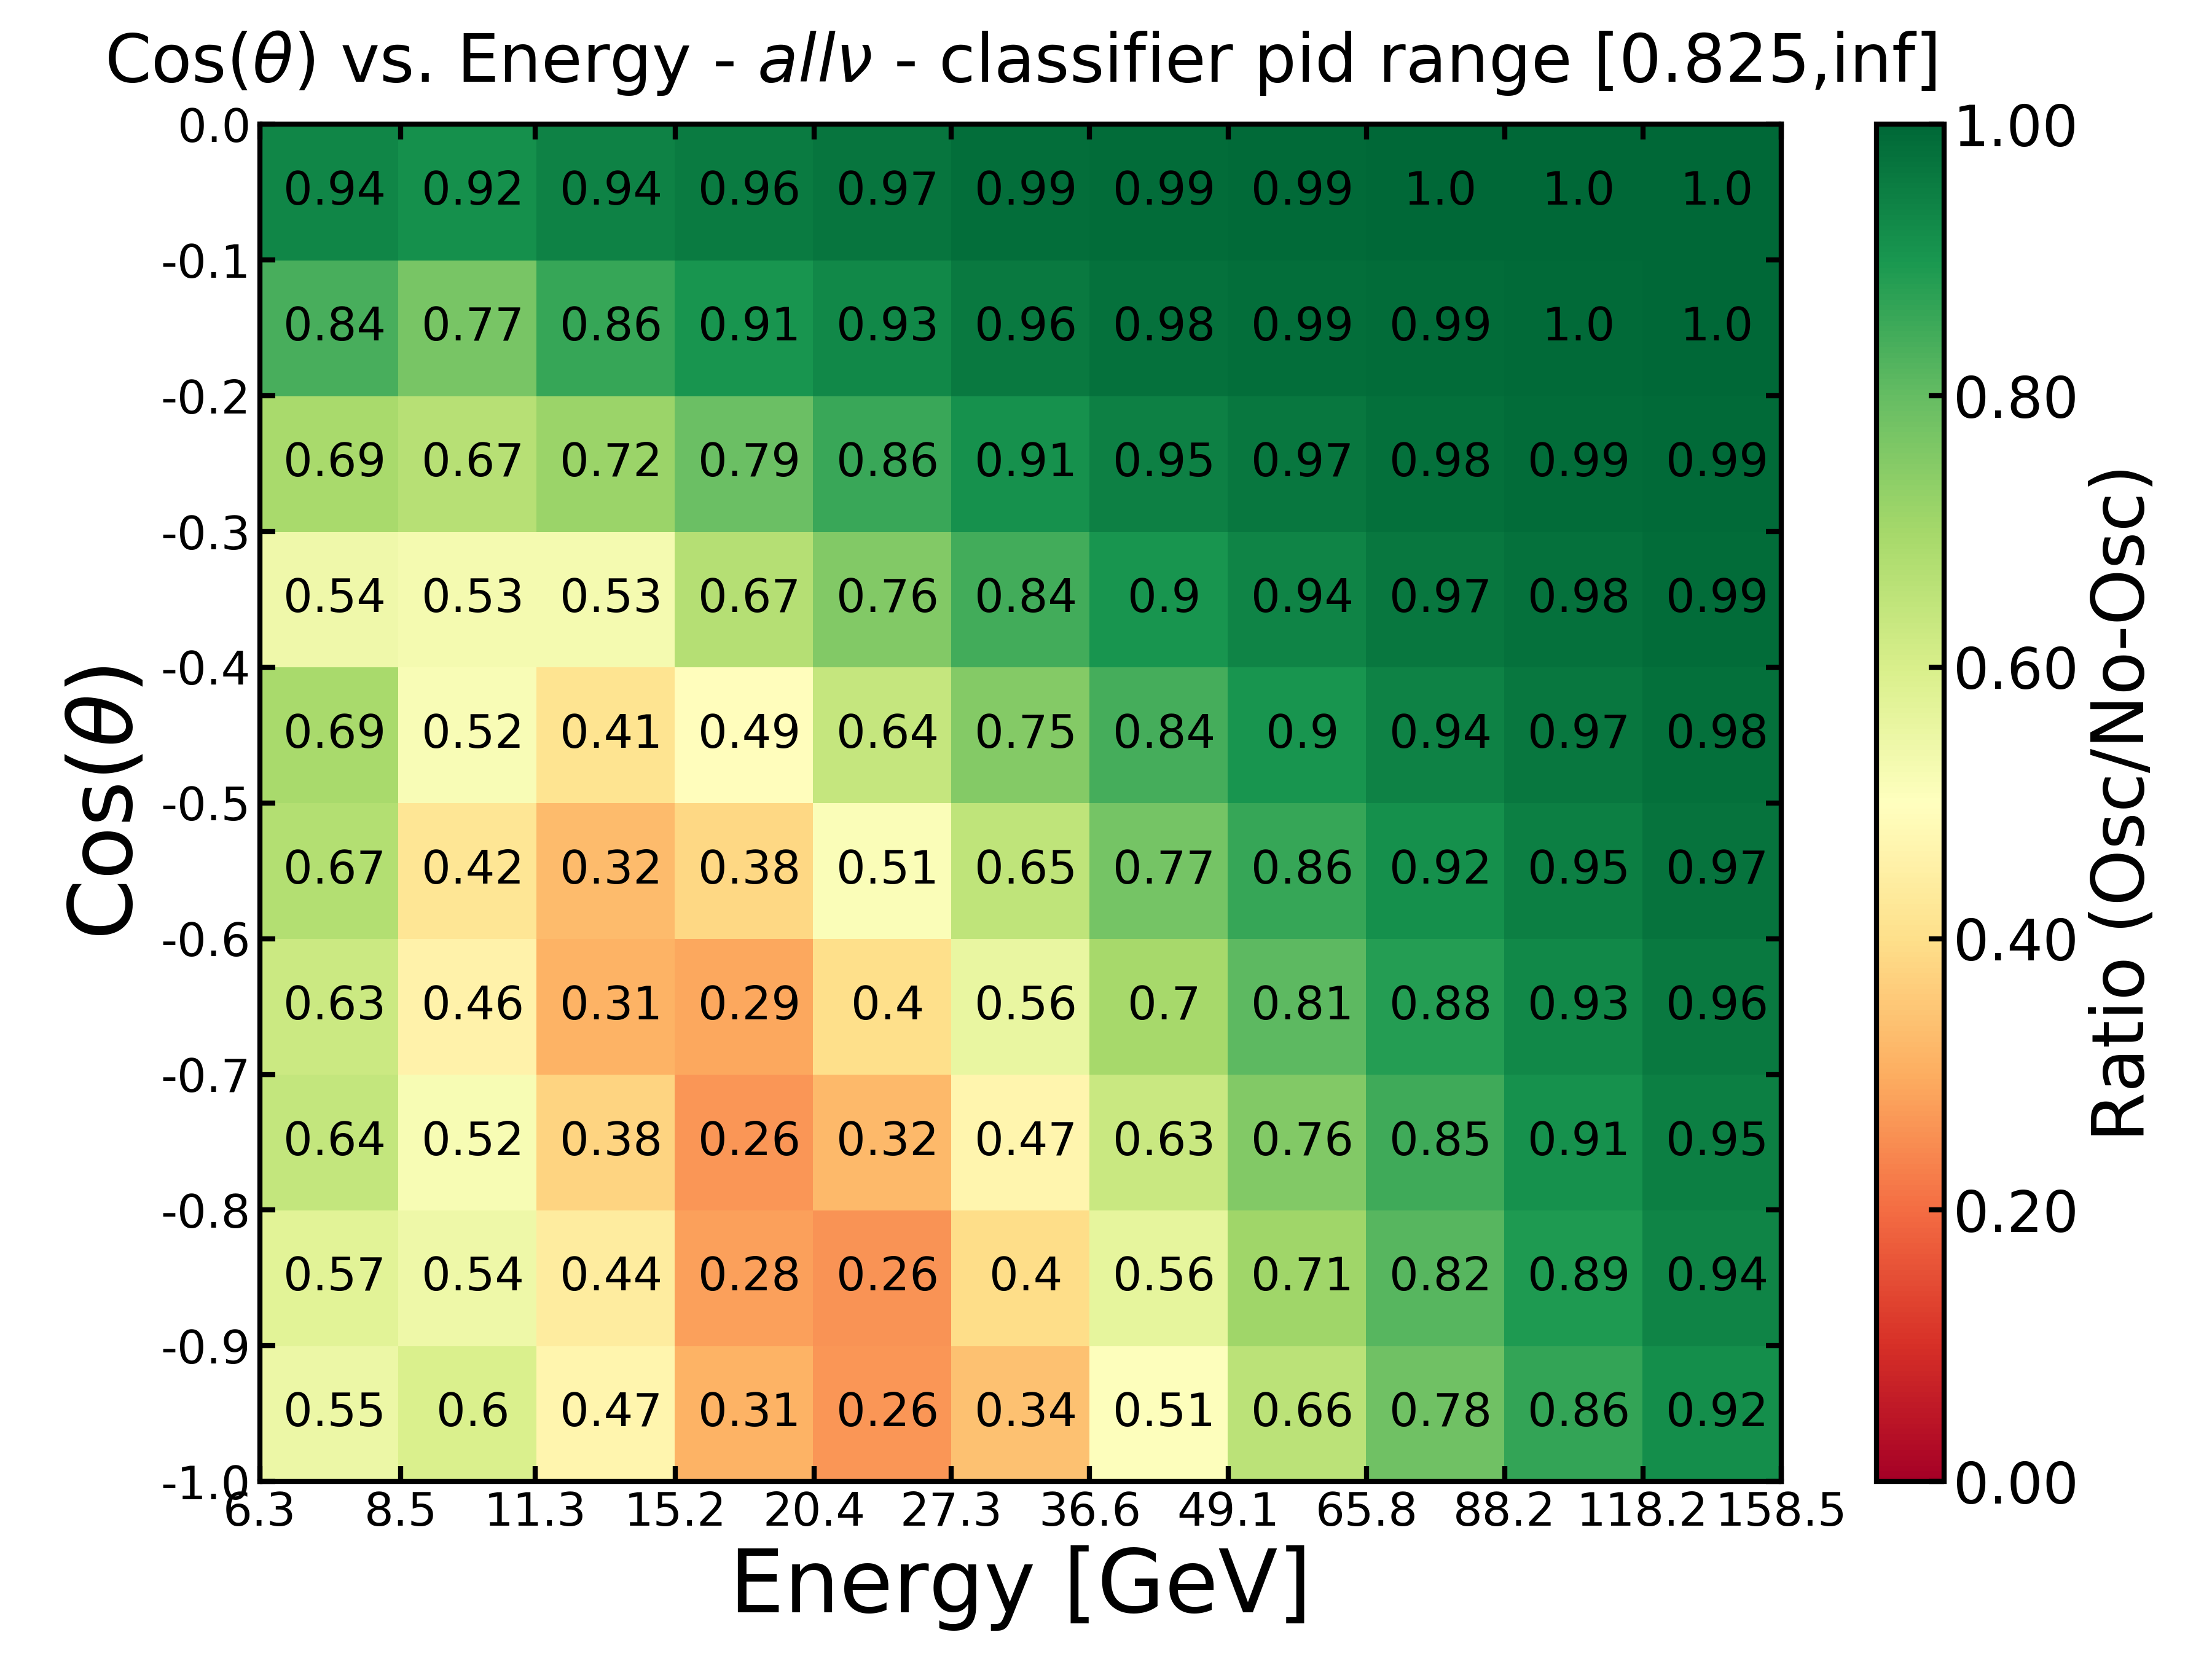
\includegraphics[width=0.49\linewidth]{figures/three_bin_cut_0575_0825_allnu_2_ratio_osc_noosc.png}
    \caption[Expected neutrino oscillation effects for three-bin case with GBM probability]{Expected neutrino oscillation effects for three-bin case with GBM probability. Shown is the ration between un-oscillated and oscillated event rates for the cascade bin (top left), the intermediate bin (top right) and the track bin (bottom center).}
    \label{fig:oscillation_effects_gbm_3bin}
\end{figure}

\newpage

\section{Sensitivity Improvement} \label{sec:sensitivity_improvement}

The performance of the GBM probability used with two bins and with three bins will be compared to the $\chi^2$-ratio PID with two bins by calculating the Asimov sensitivities for each case.
The same binning, livetime and mass ordering as in Section~\ref{sec:pid_optimization} is chosen, but this time the injected oscillation parameters are taken from a more recent fit \cite{Esteban2017} and the oscillation probabilities are calculated in the full three flavor model with matter effects using the algorithm from \cite{PhysRevD.22.2718, Prob3++} and PREM \cite{DZIEWONSKI1981297} as Earth matter profile.
Two sensitivity studies to atmospheric neutrino mixing are performed; one without systematic uncertainties and one including systematic uncertainties.
The values of the widths of the 68\,\% C.L. and the relative improvement compared to the study using the $\chi^2$-ratio PID are listed in Table~\ref{tab:sensitivity_improvement_nosyst}.
The result using two bins with the GBM probability shows marginal improvement in the sensitivity in the mass splitting.
The version using three bins shows better performance for both the mass splitting and the mixing angle, reducing the uncertainty by 8.7\,\% and 3.1\,\%, respectively.

\begin{table}[h]
    \centering
    \begin{tabular} { l || c | c | c | c}
        & $\Delta(\Delta \mathrm{m}^{2}_{32})\,[10^{-5}\mathrm{eV}^2]$ & improv.\,[\%] & $\Delta(\sin^{2}(\theta_{23}))\,[10^{-2}]$ & improv.\,[\%] \\
        \hline \hline 
        $\chi^2$-ratio PID - 2 bins & 3.67  & NA & 6.46  & NA \\
        GBM probability - 2 bins & 3.49 & 4.9 & 6.43 & 0.6 \\
        GBM probability - 3 bins & 3.35  & 8.7 & 6.26 & 3.1 \\
    \end{tabular}
    \caption[Sensitivity improvement results for the study without systematics]{Sensitivity improvement results for the study without systematics. Improvement is the relative fraction compared to the sensitivity using $\chi^2$-ratio as PID. $\Delta(\Delta \mathrm{m}^{2}_{32})$ and $\Delta(\sin^{2}(\theta_{23}))$ are the sizes of the $68$\,\% C.L. for mixing angle and mass splitting, respectively.}
    \label{tab:sensitivity_improvement_nosyst}
\end{table}

The same procedure is performed including systematic uncertainties and the results are summarized in Table~\ref{tab:sensitivity_improvement_fluxsyst}.
The results show a similar trend.
For the two-bin version there is significant improvement in both quantities, but it is much stronger in the mass splitting.
Splitting the sample in three bins based on the GBM probability leads to a larger improvement in the sensitivities of the mass splitting and the mixing angle, but the effect is stronger on the mixing angle.

\begin{table}[h]
    \centering
    \begin{tabular} { l || c | c | c | c}
        & $\Delta(\Delta \mathrm{m}^{2}_{32})\,[10^{-5}\mathrm{eV}^2]$ & improv.\,[\%] & $\Delta(\sin^{2}(\theta_{23}))\,[10^{-2}]$ & improv.\,[\%] \\
        \hline \hline 
        $\chi^2$-ratio PID - 2 bins & 4.97 & NA & 7.65 & NA \\
        GBM probability - 2 bins & 4.50 & 9.5 & 7.41 & 3.1 \\
        GBM probability - 3 bins & 4.32 & 13.0 & 7.10 & 7.2 \\
    \end{tabular}
    \caption[Sensitivity improvement results for the study including systematics]{Sensitivity improvement results for the study including systematics. Improvement is the relative fraction compared to the sensitivity using $\chi^2$-ratio as PID. $\Delta(\Delta \mathrm{m}^{2}_{32})$ and $\Delta(\sin^{2}(\theta_{23}))$ are the sizes of the $68$\,\% C.L. for mixing angle and mass splitting, respectively.}
    \label{tab:sensitivity_improvement_fluxsyst}
\end{table}

The best results are achieved using the GBM probability PID with three bins which yields $\Delta(\Delta \mathrm{m}^{2}_{32}) = 4.32\cdot10^{-5}\,\mathrm{eV}^2$ and $\Delta(\sin^{2}(\theta_{23})) = 7.10\cdot10^{-2}$.
This is a 13.0\,\% improvement in $\Delta(\Delta \mathrm{m}^{2}_{32})$ and a 7.2\,\% improvement in $\Delta(\sin^{2}(\theta_{23})) = 7.10\cdot10^{-2}$ relative to the uncertainties estimated using the $\chi^2$-ratio PID.
The improvement that can be achieved by applying the new PID variable demonstrates the strength of the multivariate classification algorithm.
As compared to the formerly used univariate discriminator, the new discriminator maximizes the use of information gained from the set of input variables.
